\chapter[REFERENCIAL TEÓRICO]{REFERENCIAL TEÓRICO}

Esta seção visa oferecer uma os conceitos básicos para o entendimento deste trabalho de pesquisa. Inicialmente será mostrado a categoria de pequenos satélites e a concepção do padrão CubeSat. Logo em seguida, será exposto os principais subsistemas de um CubeSat, dando ênfase no computador de bordo. Será mostrado a importância do barramento PC104 e as interferências do ambiente espacial em sistemas embarcados.


\section{Pequenos Satélites}

O termo “pequenos satélites” é designado para caracterizar satélites que possuem massa úmida (massa do satélite mais massa do propelente) inferior a 500 kg. Esta definição cumpre a terminologia estabelecida pelo \textit{Small Space Technology Program} (SSTP) da NASA (FROST; AGASID, 2015). As subcategorias de pequenos satélites, e alguns exemplos de espaçonaves já lançadas, podem ser observadas na figura abaixo.


\begin{figure}[h]
	\centering
    {\small\caption{Categoria de Pequenos Satélites e alguns exemplos.}}
	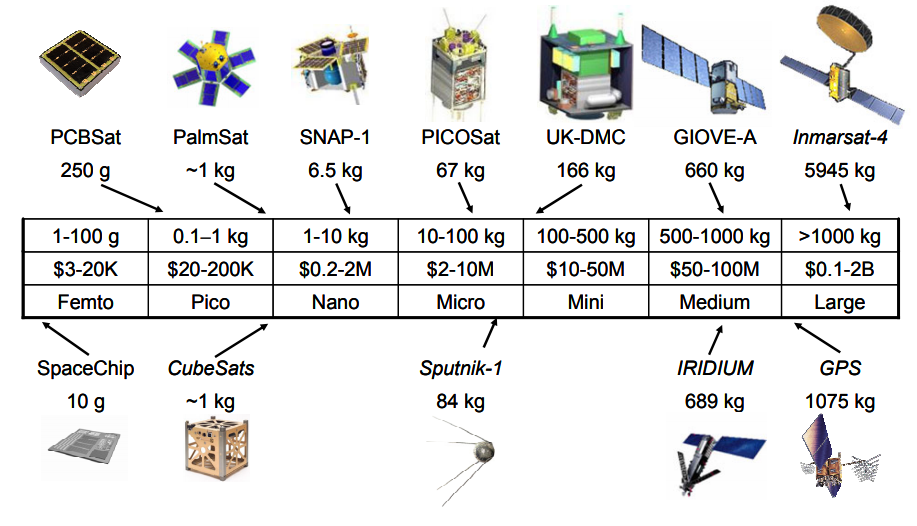
\includegraphics[keepaspectratio=true,scale=0.55]{figuras/categoria_satellite.PNG}
	Fonte:(BARNHART, 2008, pág.42).
	\label{fig02}
\end{figure}


As espaçonaves são normalmente agrupadas conforme sua massa. Como visto na figura acima, pequenos satélites podem ser divididos nas seguintes subcategorias: minissatélites com massa entre 100-500kg, microsatélites com massa entre 10-100kg, nanosatélites com massa entre 1-10kg, picosatélites com massa entre 0.1-1kg e femtosatélites com massa entre 1-100g. No limite superior dessa categoria, existem minisatélites como o Globalstar, satélite de telecomunicações da empresa Globalstar LP, que possui massa úmida de 450kg (GLOBALSTAR, L.P, 2000). Já no extremo inferior, existem projetos como o KickSat que colocou em órbita 128 femtosatelites  com 5g (GRIFFITHS, 2017).

Nas últimas décadas, houve um aumento no lançamento de nanosatélites. Esse crescimento pode ser observado na Figura \ref{fig03}, que mostra a quantidade de pequenos satélites colocados em órbita entre os anos de 1995 e 2014. Fatores como a miniaturização da eletrônica, otimização dos veículos lançadores e crescimento de empresas no setor ajudaram nesse crescimento (FACCHINETTI et al., 2016).

{\small
\begin{figure}[h]
	\centering
	\caption{Lançamento de pequenos satélites entre 1995 e 2014.}
	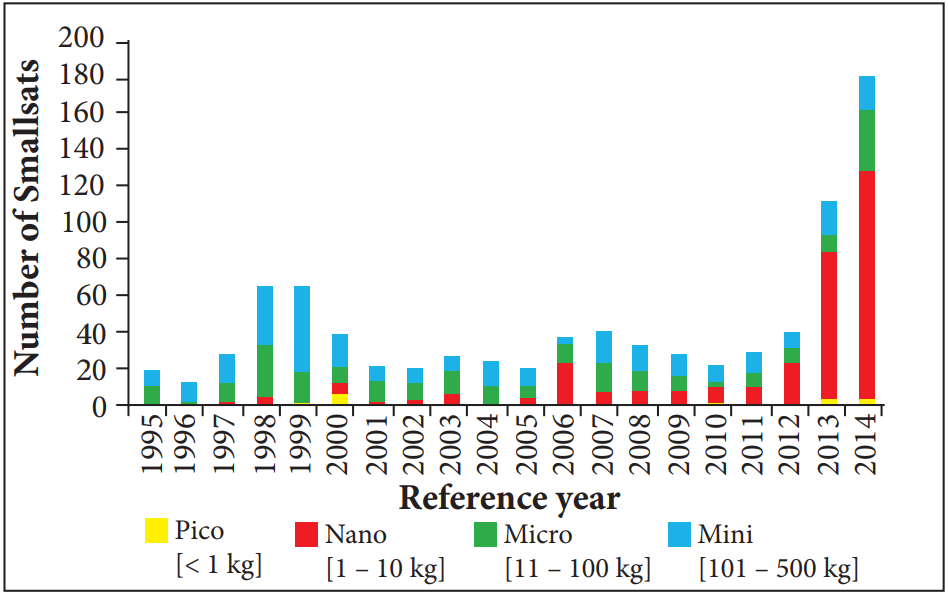
\includegraphics[keepaspectratio=true,scale=0.55]{figuras/lancamentoPequenoSatellite.PNG}
	Fonte:(WEKERLE; FILHO, 2017, pág.3).
	\label{fig03}
\end{figure}
}

Fazendo uma análise minuciosa nos sites Nanosatellite Database\footnote{ KULU, Erik. Nanosatellite Database by Erik. 2018. Disponível em: \url{http://www.nanosats.eu/}. Acesso em: 14 maio 2018.} e Space Launch Report\footnote{N2YO. Browse Satellites by Launch date. 2018. Disponível em:\url{https://www.n2yo.com/browse/}.  Acesso em: 14 maio 2018.}, sites que armazenam dados de missões satelitais, observa-se que em 2007 cerca de 2,6\%(9 de 348 satélites) eram CubeSats. Já em 2017 o numero de lançamentos passou para 57,6\% (295 de 512 satélites). Tendo como base esses valores, pode-se afirmar que os CubeSats ajudaram a popularização da categoria de nanosatélites.

De forma resumida, o CubeSat é um satélite cúbico de 10 cm de aresta e que pesa apenas alguns quilogramas, sendo muito utilizado no meio acadêmico. Eles podem ser compostos por um único cubo (uma unidade ou 1U) ou vários cubos combinados formando, por exemplo, unidades 3U e 6U. A Figura \ref{fig04} mostra as configurações mais usuais de um CubeSat (FROST; AGASID, 2015).

{\small
\begin{figure}[h]
	\centering
    \caption{Algumas variações de CubeSat.}
	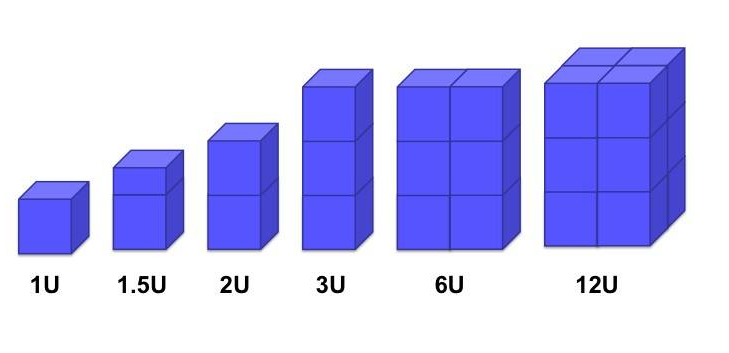
\includegraphics[keepaspectratio=true,scale=0.58]{figuras/cubesatVariacoes.PNG}	
	
	Fonte:(MABROUK, 2017, pág.1).
	\label{fig04}
\end{figure}
}

\section{Padrão CubeSat}

O padrão CubeSat começou como um esforço colaborativo entre Jordi Puig-Suari, professor na Universidade Politécnica da Califórnia (CalPoly), e Bob Twiggs, professor na Universidade de Stanford. A intenção original era fornecer para a comunidade científica universitária meios mais acessíveis ao espaço (DEEPAK; TWIGGS, 2012).

Twiggs retrata o contexto histórico do desenvolvimento do conceito CubeSat em detalhes no seu artigo “\textit{Origin of CubeSat}” (TWIGGS, 2008). Em resumo, o abandono radical do design tradicional de satélites, ocasionado pelo CubeSat, começou após o lançamento bem-sucedido do \textit{Orbiting Picosatellite Automatic Launcher} (OPAL), projeto liderado por Twiggs, que pôs em órbita seis \textit{hockey} picosatélites. Inspirado por esse sucesso, Twiggs explorou um \textit{design} maior e mais cúbico para suportar mais capacidade. Ele encontrou o modelo perfeito para seu novo \textit{design} em uma loja varejo, uma embalagem cúbica de 10 cm para ursinhos de pelúcia. O nanosatélites resultante foi um cubo medindo 10 cm de aresta e pesando apenas 1 kg, nomeado CubeSat (DEEPAK; TWIGGS, 2012).

Mais tarde naquele ano, Twiggs e Puig-Suari disponibilizaram as especificações para o Padrão CubeSat. Em 2003, Puig-Suari e CalPoly desenvolveram o \textit{Poly-PicoSatellite Orbital Deploye} (P-POD) para lançar até três CubeSats 1U. As primeiras missões CubeSat começaram no  mesmo ano do desenvolvimento do P-POD (DEEPAK; TWIGGS, 2012).

Com o passar dos anos, a documentação do \textit{CubeSat Standard} sofreu algumas alterações. A versão mais atualizada pode ser encontrada em alguns sites, como o Cubesat.org\footnote{CubeSat INFO. 2018. Disponível em:\url{https://goo.gl/P8vZYy}. Acesso em: 14 maio 2018.}. A Figura \ref{fig05} mostra as dimensões padronizadas de um CubeSat 3U+ (CUBESAT PROGRAM, 2014). Um ponto a ser mencionado é que o 3U+ foi criado para atender as demandas de sensoriamento remoto, possibilitando colocar uma câmera sem prejudicar o espaço interno da plataforma.

{\small
\begin{figure}[h]
	\centering
    \caption{Especificações Estruturais para um CubeSat 3U+.}
	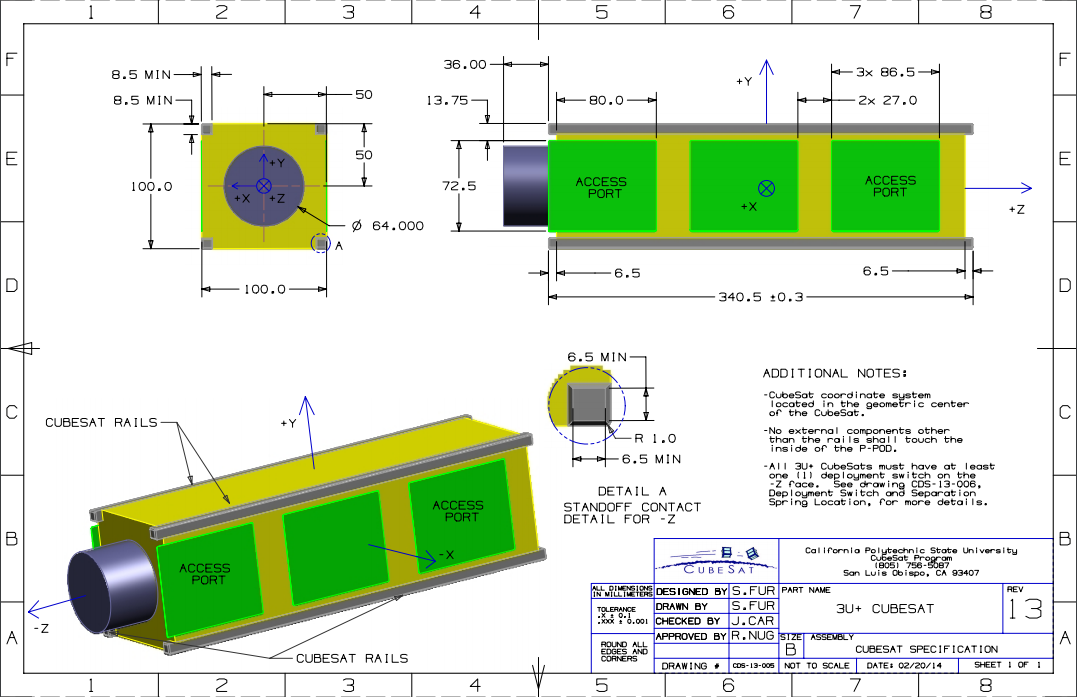
\includegraphics[keepaspectratio=true,scale=0.55]{figuras/cubesat3u+.PNG}
	
	Fonte:(CUBESAT PROGRAM, 2014, pág.31).
	\label{fig05}
\end{figure}
}

Graças aos CubeSats, muitas universidades possuem seu próprio programa espacial. Porém, o uso dessa tecnologia não é exclusiva apenas para grandes universidades; escolas secundárias, ensino médio e escolas primárias puderam desenvolver suas próprias missões (DEEPAK; TWIGGS, 2012). Um exemplo de projeto é o UbatubaSat, CubeSat feito pelos estudantes da escola municipal Tancredo de Almeida Neves, em Ubatuba-SP (FIORAVANTI, 2011).

Essa facilidade de acesso ao espaço é consequência de algumas características que o padrão CubeSat dispõem. De acordo com a empresa ISIS (2018), esses aspectos podem ser sintetizados em sete atributos:

\begin{itemize}

	\item \textbf{Modularidade}: Por possuir um tamanho normatizado, tornou-se possível desenvolver módulos funcionais padronizados, como subsistemas de energía, comunicação, entre outros. Esse aspecto fez com que soluções de prateleira (COTS, do inglês \textit{Commercial Off-The-Shelf}) fossem amplamente utilizadas no projeto de algumas missões, agilizando e barateando o desenvolvimento do CubeSat;

	\item \textbf{Lançamento}: Os CubeSats são tipicamente lançados no espaço como cargas contidas em contêineres padronizados, por exemplo, P-POD, visando a redução da complexidade e custo do lançamento;
	\item \textbf{Custo}: Geralmente as missões CubeSat são desenvolvidas usando um "orçamento baixo", comparado às missões tradicionais;
    \item \textbf{Componentes}: Componentes que não possuem o selo “\textit{Space Qualified}” são frequentemente utilizados e aceitos em missões CubeSat, permitindo uma abordagem de baixo custo e de rápida implementação. O fato de muitas missões CubeSat estarem em órbita baixa e possuírem um tempo de vida curto faz com que o uso desses componentes se torne viável;
    \item \textbf{Desenvolvimento}: Devido à baixa complexidade e escopo limitado, é comum usar metodologias de projeto menos formais. Em algumas circunstâncias, é possível trabalhar em equipes compactas, eliminando a necessidade de pacotes de documentação e outras despesas gerais. Obviamente, um nível mínimo de formalidade e documentação é sempre necessário;
    \item \textbf{Risco}: Tipicamente, a abordagem utilizada em missões CubeSats correm um risco técnico mais elevado oferecendo em troca: custo menor, implementação mais rápida, aplicação mais inovadora, ou um conjunto desses elementos;
    \item \textbf{Nichos de Aplicação}: O benefício do padrão CubeSats não é possuir boa performance em termo de largura de banda ou resolução espacial, pois não é compatível com as restrições estruturais impostas pelo padrão. Entretanto, quando usado em redes ou constelações, os CubeSats são capazes de fornecer uma resolução temporal a preços acessíveis.

\end{itemize}

\section{Principais Subsistemas de um CubeSat}

Os CubeSats são formados por duas partes principais, que são: a Carga Útil (do inglês \textit{Payload}) e a plataforma (chamada em inglês de \textit{Bus}). A Carga Útil é definida de acordo com a missão do satélite, por exemplo: satélites para observação da Terra possuem como carga útil uma câmera; satélites para telecomunicações possuem um rádio; etc. A Plataforma tem o objetivo de abrigar a Carga Útil para que ela funcione normalmente no ambiente espacial. A Plataforma é geralmente composta por: Sistema Estrutural (SS, do inglês \textit{Structural System}), Sistema de Potência Elética (EPS, do inglês \textit{Electrical Power System}), Sistema de Controle e Determinação de Órbita \& Atitude (AODCS,do inglês \textit{Attitude and Orbit Determination and Control System}), Controle de Telecomando e Telemetria (TT\&C, do inglês \textit{Telemetry Telecomand Control}) e o Computador de Bordo (OBC, do inglês \textit{On-Board Computer}). 

A Figura \ref{fig06} visa ilustrar esses subsistemas (ADDAIM; KHERRAS; ZANTOU, 2010).

\begin{figure}[h]
	\centering
    \caption{Arquitetura de um Satélite.}
	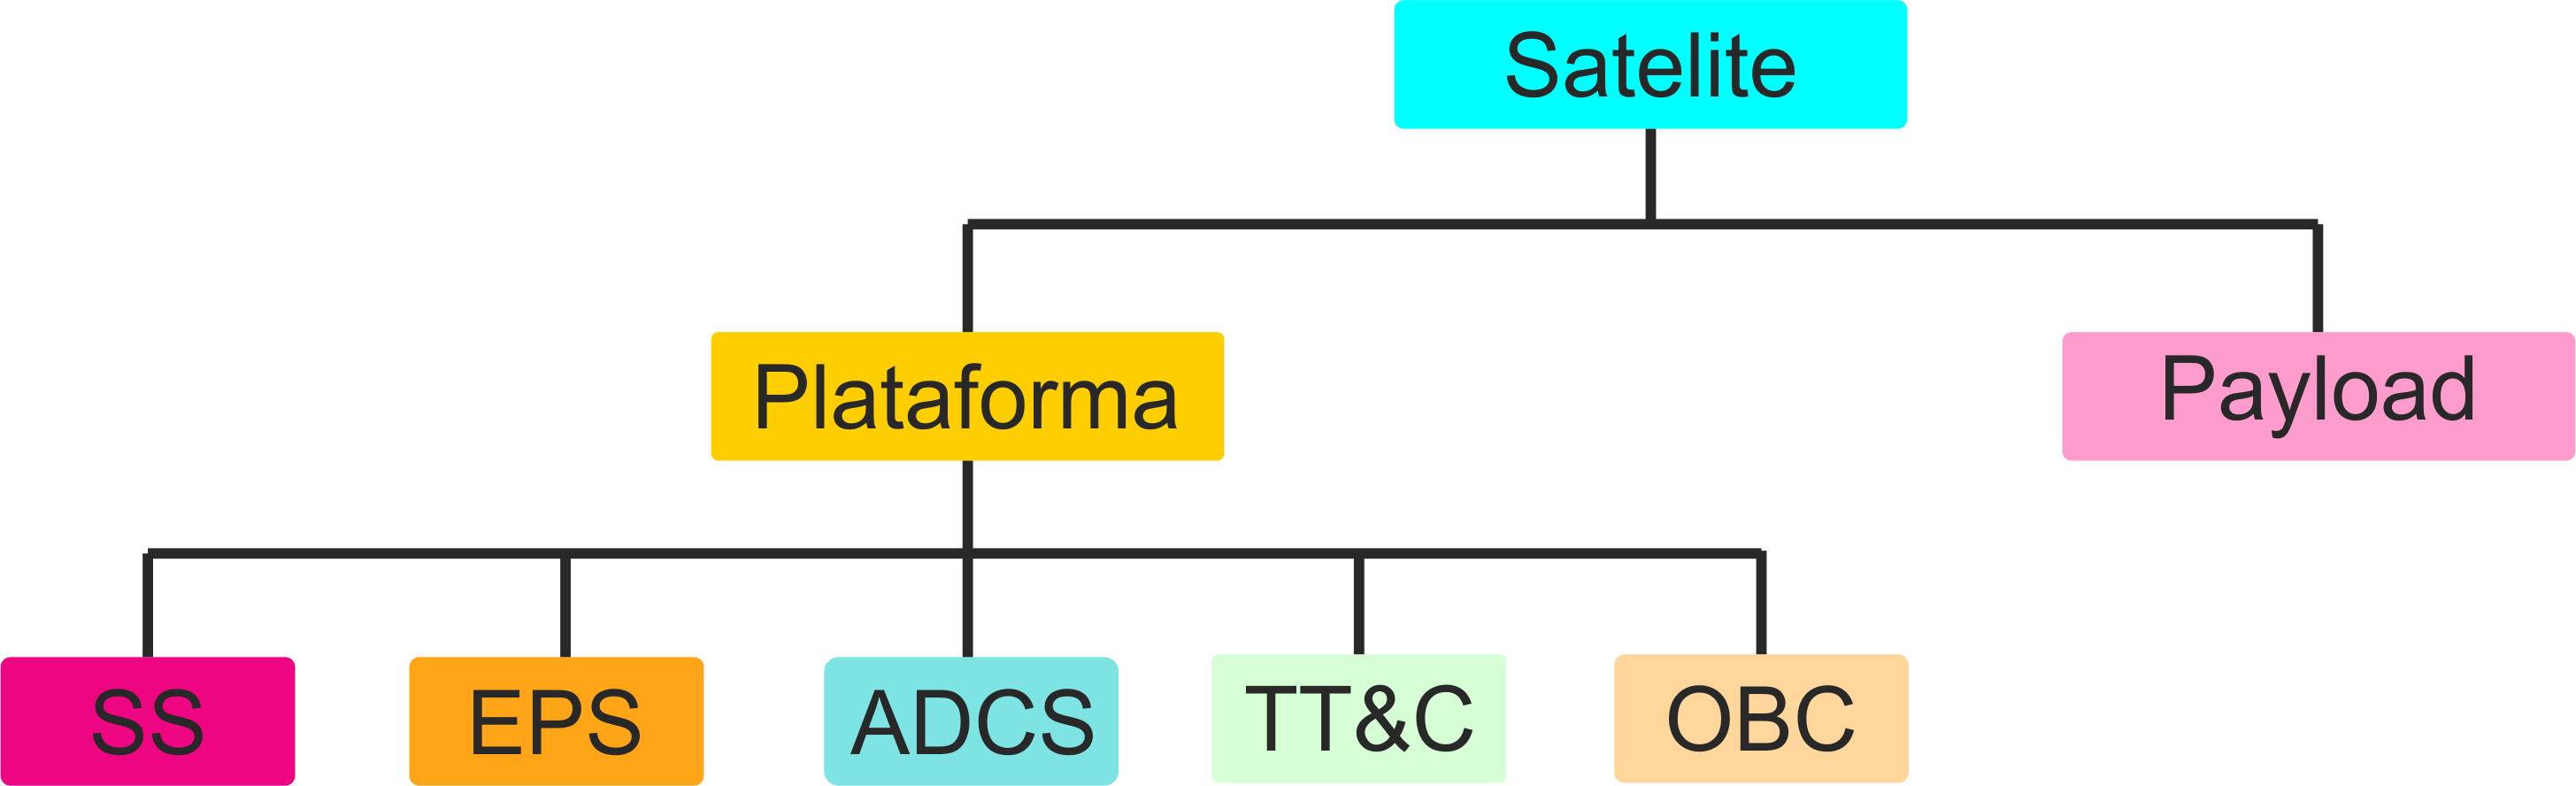
\includegraphics[keepaspectratio=true,scale=0.5]{figuras/estrutura_satellite.png}
	
	Fonte:(ADDAIM; KHERRAS ; ZANTOU, 2010, adaptado pág.6).
	
	\label{fig06}
\end{figure}

\newpage

Abaixo há uma breve descrição dos subsistemas e alguns exemplos de componentes comerciais.

\textbf{Descrição dos Subsistemas:}

\begin{itemize}

	\item \textbf{SS}: Esse subsistema visa proteger o satélite dos efeitos do ambiente espacial e servir como interface com o veículo lançador. O SS deve ser leve e resistente, sem contar que deve blindar ao máximo a radiação espacial. Geralmente o material utilizado na estrutura é alguma liga de alumínio.  A Figura \ref{fig07} mostra o \textit{Structure Subsystem} da NanoAvionics\footnote{Empresa NanoAvionics. 2018. Disponível em:\url{https://n-avionics.com/}. Acesso em: 30 maio 2018.}.

\begin{figure}[h]
	\centering
    \caption{Estrutura 3U Padrão NanoAvionics.}
    
	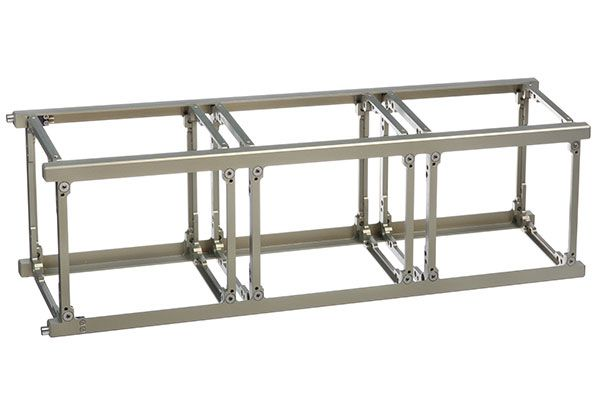
\includegraphics[keepaspectratio=true,scale=0.4]{figuras/cubesat-structure-main.jpg}
	
	Fonte:(NANO AVIONICS, 2018, pág.1).\linebreak
	
	\label{fig07}
\end{figure}

	\item \textbf{EPS}: O \textit{Electrical Power System} tem o objetivo de fornecer energia elétrica à todos os subsistemas, inclusive a carga útil. Ele é responsável pela geração, armazenamento e distribuição da energia elétrica. Os principais elementos de um EPS são: baterias, painéis solares e switchs. A Figura \ref{fig08} é mostra os principais elementos de um EPS.
    
\begin{figure}[h]
	\centering
    \caption{Principais componentes de um EPS.}
	
	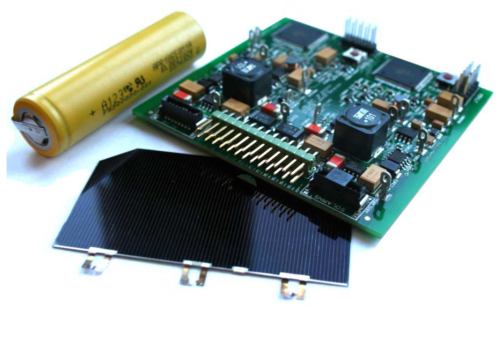
\includegraphics[keepaspectratio=true,scale=1.5]{figuras/eps.png}
	
	Fonte:(CUBESTAR, 2018, pág.1).\linebreak
	
	\label{fig08}
\end{figure}

\newpage
	\item \textbf{AODCS}: Esse subsistema tem o objetivo de garantir que câmeras e antenas estejam apontados para os alvos predeterminados. Os principais componentes do AODCS são: rodas de reação, sensores inerciais, fotodiodos  e magnetorques. Recentemente estão sendo utilizados módulos PPT (\textit{Pulsed Plasma Thruster}) para compensar o arrasto atmosférico. A Figura \ref{fig09} é mostra o AODCS (esquerda)  e PPT (direita) da empresa Clyde Space\footnote{Empresa Clyde Space. 2018. Disponível em:\url{https://www.clyde.space/}. Acesso em: 30 maio 2018.}.

\begin{figure}[h]
	\centering
    \caption{Componentes AODCS da empresa Clyde Space.}
    
	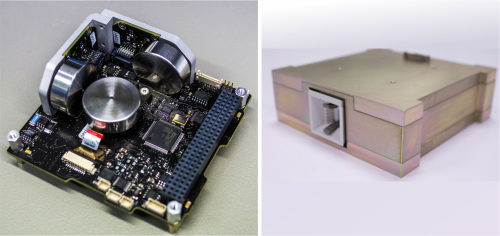
\includegraphics[keepaspectratio=true,scale=2.2]{figuras/aodcs.png}
	
	Fonte: (CLYDE SPACE, 2018, pág.1).\linebreak
	
	\label{fig09}
\end{figure}

    \item \textbf{TT\&C}: Esse subsistema serve como interface entre a estação de solo e o Satélite. Ele envia pacotes de telemetria e dados da \textit{Payload}, e recebe telecomandos da estação terrestre. Os componentes principais desse subsistema são: transceptor e antena. A Figura \ref{fig10} mostra uma antena (esquerda) e um módulo de telecomunicações (direita) da empresa Endurosat\footnote{Empresa EnduroSat. 2018. Disponível em:\url{https://www.endurosat.com/}. Acesso em: 30 maio 2018.}.

\begin{figure}[h]
	\centering
    \caption{Componentes TT\&C da empresa EnduroSat.}
    
	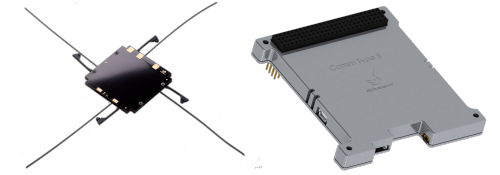
\includegraphics[keepaspectratio=true,scale=2.2]{figuras/tt_c.png}
	
	Fonte:(ENDUROSAT, 2018a).\linebreak
	
	\label{fig10}
\end{figure}

\newpage
    \item \textbf{OBC}: O satélite precisa de um subsistema capaz de gerenciar todos os outros subsistemas. O OBC tem o intuito de garantir o funcionamento de todos os subsistemas de acordo com os telecomandos, provindos da estação de solo, e do software embarcado. Os principais componentes são: microcontrolador, sistema operacional e módulo de armazenamento.  A Figura \ref{fig11} mostra o OBC da empresa EnduroSat.

\begin{figure}[h]
	\centering
  	
  	\caption{Computador de bordo da empresa EnduroSat.}
  	
	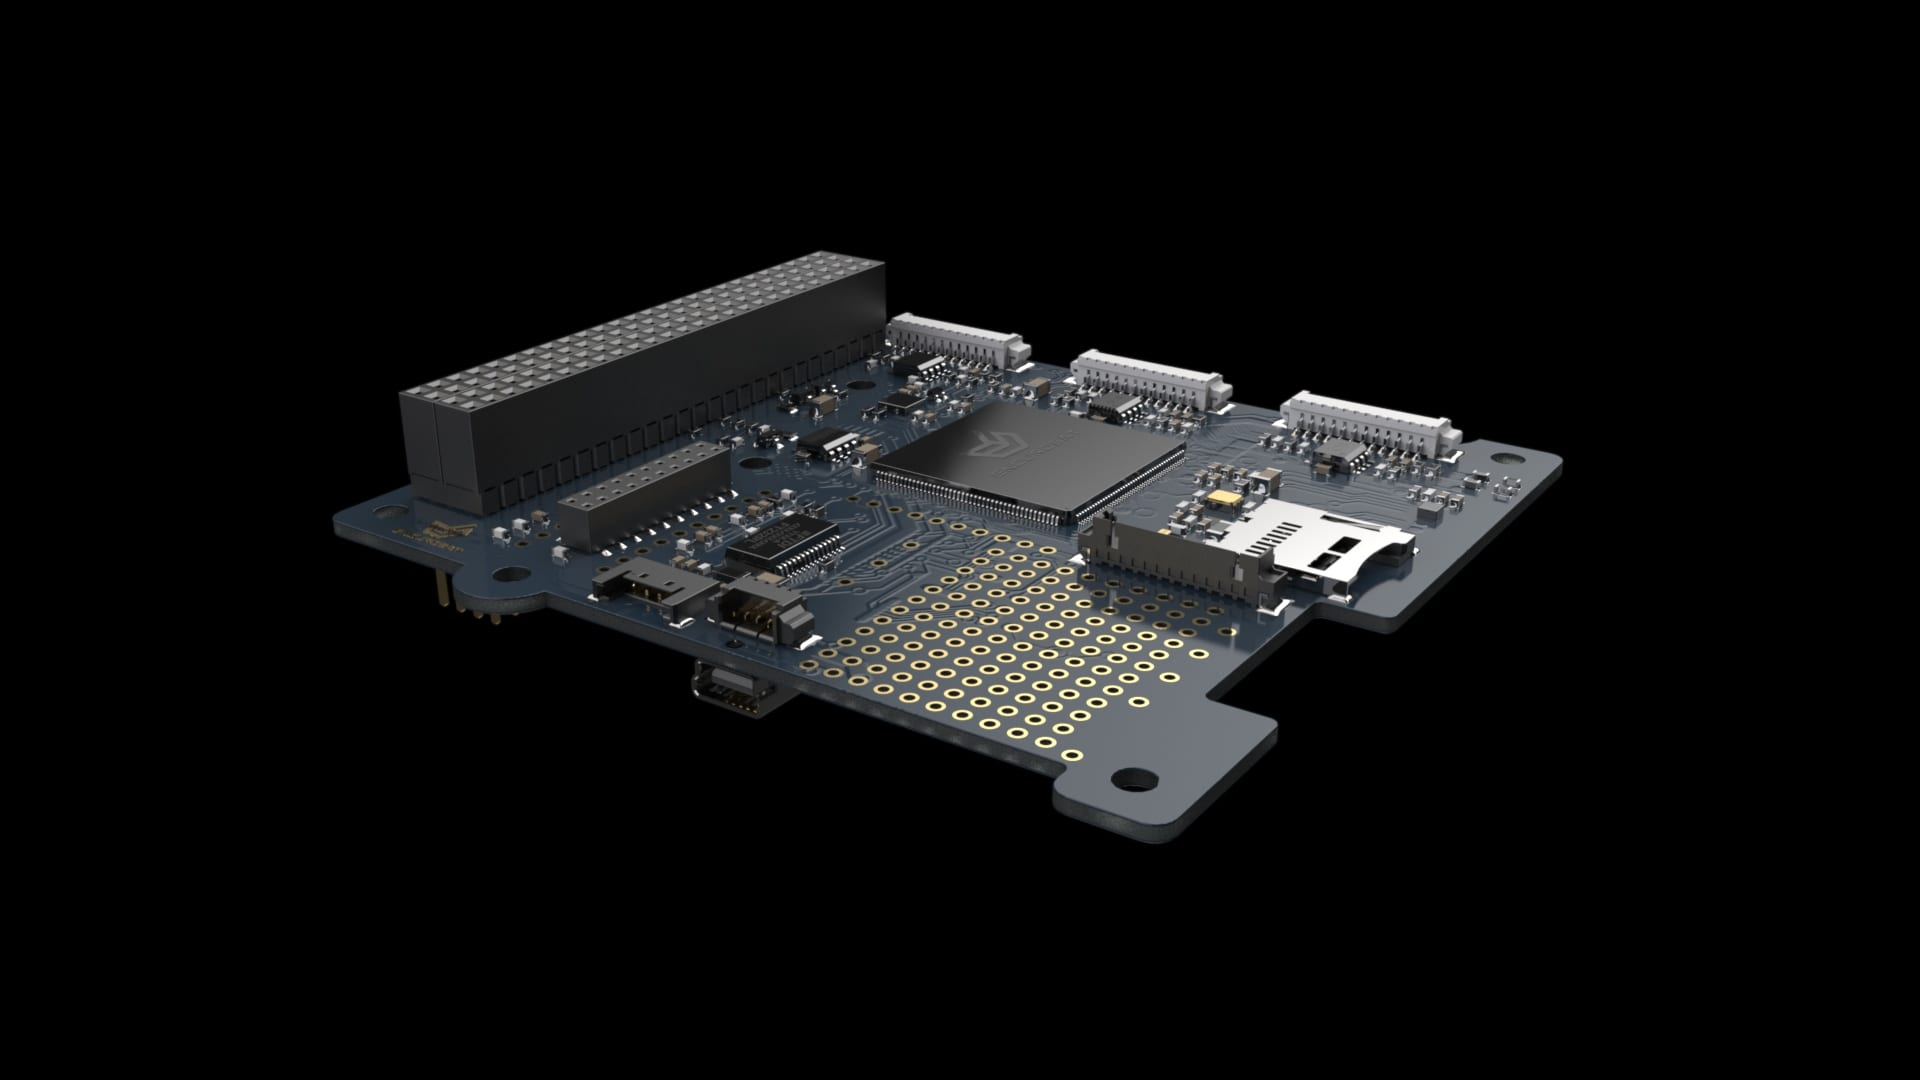
\includegraphics[keepaspectratio=true,scale=0.2]{figuras/Cubesat-OBC-module-1.jpg}
	
	Fonte:(ENDUROSAT, 2018b, pág.1).
	
	\label{fig11}
\end{figure}

\end{itemize}

\section{Visão Geral de um OBC}

O Computador de Bordo é considerado o cérebro do CubeSat e consiste, essencialmente, de um microcontrolador conectado à outros subsistemas por barramentos  e periféricos de dados. Normalmente, um Sistema Operacional de Tempo Real (RTOS, do inglês \textit{Real-Time Operating System}) controla todas as aplicações que são executadas no microcontrolador (LUMBWE, 2013).

As funções mais importantes de um OBC são exemplificadas abaixo (STRAS et al., 2003):

\begin{itemize}

\item Capturar e armazenar dados da telemetria e \textit{Payload};

\item Codificar e transmitir dados à estação de solo;

\item Processar os telecomandos provenientes da estação de solo, compensando o tempo atraso no canal de uplink;

\item Monitorar os subsistemas do Satélite.

\end{itemize}

\subsection{Computadores de Bordo Existentes}

Essa avaliação tem como objetivo mostrar ao leitor alguns OBCs, utilizados em missões CubeSat, e destacar as características mais relevantes. Uma coleta mais detalhada foi realizada e se encontra no Apêndice \ref{apendicea}.

\begin{itemize}

\item \textbf{FloripaSat OBDH}

	O projeto FloripaSat, da Universidade Federal de Santa Catarina (UFSC), possui um  computador de bordo que é responsável pela sincronização de ações e fluxo de dados entre os subsistemas (\textit{Payload} e EPS) e com a Segmento Terrestre. Esse subsistema é composto por seis submodulos: CPU (MCU: CPU + RAM + \textit{Program Flash}), memória não volátil, \textit{Driver}s de controle, unidade de medição inercial (IMU), Sensores de Corrente (sensor de Sol) e interfaces de comunicação (FLORIPASAT,2016).

	O sistema responsável pela execução do \textit{firmware} consiste de SoC que contém uma CPU, Memória RAM e Flash (usado para armazenamento de programas e status dos registradores). O Microcontrolador escolhido foi o MSP430F6659IPZ da Texas Instruments. Tal microcontrolador, conhecido por ter um baixo consumo, possui sete modos de operação de consumo, 4 timers de 16-bits, 12 AD/DA de 12-bits, 6 interfaces de comunicação serial, bloco de real-time clock (RTC) e mais de 74 pinos de I/O. O clock de operação do OBDH é de 32MHz (FLORIPASAT,2016).

	Provendo um sistema de redundância, há um monitor de tensão com um \textit{Watchdog Timer} (FLORIPASAT,2016). A Figura \ref{fig12} mostra a arquitetura do FloripaSat OBDH.

\begin{figure}[h]
	\centering
	
	\caption{Arquitetura do OBDH do FloripaSat.}
	
	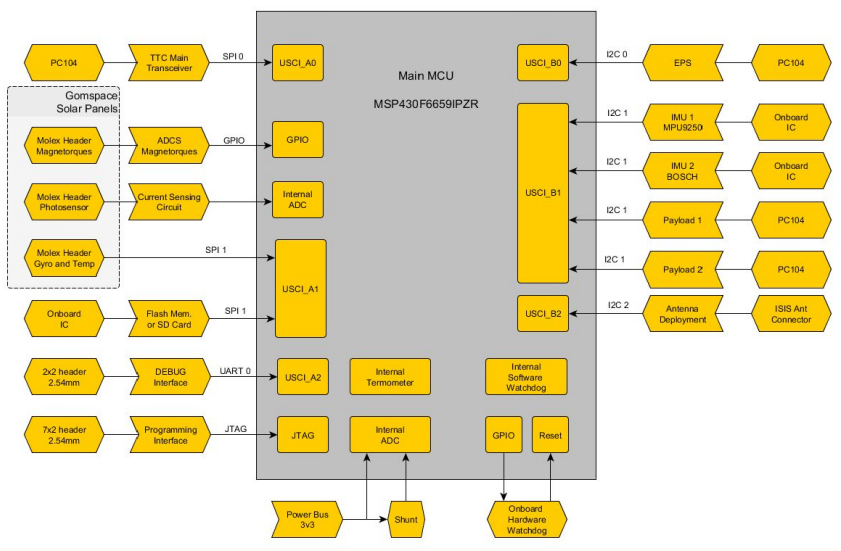
\includegraphics[keepaspectratio=true,scale=0.5]{figuras/floripasatobdh.PNG}
	
	Fonte: (FLORIPASAT,2016, pág.45).\linebreak
	
	\label{fig12}
\end{figure}

\newpage
\item \textbf{Open OBC}

Esse é um computador open source para CubeSat, desenvolvido pela Universidade Federal do Ceará (UFC) com o do Instituto Nacional de Pesquisas Espaciais (INPE), tendo como pontos fortes o baixo custo e a ata confiabilidade. A arquitetura utilizada no Open OBC  contém: processador TMS570LS0432 da fabricante Texas Instruments.

A arquitetura proposta utiliza o processador TMS570LS0432 do fabricante Texas Instruments, o qual possui: núcleo ARM Cortex-R4 em duas CPUs; detecção e correção de falhas em suas memórias RAM e ROM internas; \textit{hardware} BIST (Auto-teste interno de fábrica) tanto na CPU quanto na memória RAM; e outras características de segurança como o monitoramento do clock e da tensão de alimentação. Uma memória \textit{Flash} externa foi utilizada para armazenamento de código e dados. Foram disponibilizadas duas interfaces I2C para a comunicação com os subsistemas existentes em um CubeSat, sendo uma exclusiva para comunicação com o Transponder e outra comum para os demais. A arquitetura é complementada por uma interface UART para diagnóstico e depuração, sinais PWM para acionamento das bobinas de torque e entradas ADC para medição da intensidade da luz solar nas faces do satélite. Estão previstos ainda um cartão MicroSD para armazenamentos de dados e uma interface CAN para tráfego de informações transmitidas em tempo real, garantindo assim um controle rígido de erros e a recepção de mensagens (OPENOBC, 2017).

\begin{figure}[h]
	\centering
    \caption{Arquitetura do OpenOBC.}
    
	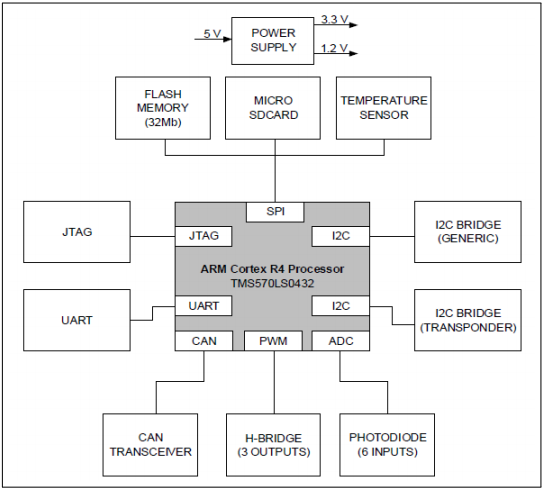
\includegraphics[keepaspectratio=true,scale=0.55]{figuras/openObc.PNG}
	
	Fonte: (OPENOBC, 2017, pág.28). \linebreak
	
	\label{fig13}
\end{figure}

\newpage

\item \textbf{ISIS On Board Computer (iOBC)}

O iOBC, do fabricante  ISIS (Innovative Solution In Space), é um computador de bordo com alto desempenho baseado em um processador ARM9 com velocidade de clock de 400MHz e oferece uma infinidade de interfaces padronizadas. Tem a capacidade de modularidade, permitindo a adição de eletrônicos ou interfaces específicas da missão, tornando o iOBC um ótimo computador de bordo para inúmeras missões.	A arquitetura utiliza o processador AT91SAM9G20 do fabricante Microchip, o qual possui: núcleo ARM9 32-bit com 400MHz (ISIS, 2016).

A fabricante não disponibilizou a arquitetura do iOBC. A Figura \ref{fig14} mostra a placa eletrônica do iOBC. 

\begin{figure}[h]
	\centering
    \caption{Placa Eletrônica - iOBC.}
    
	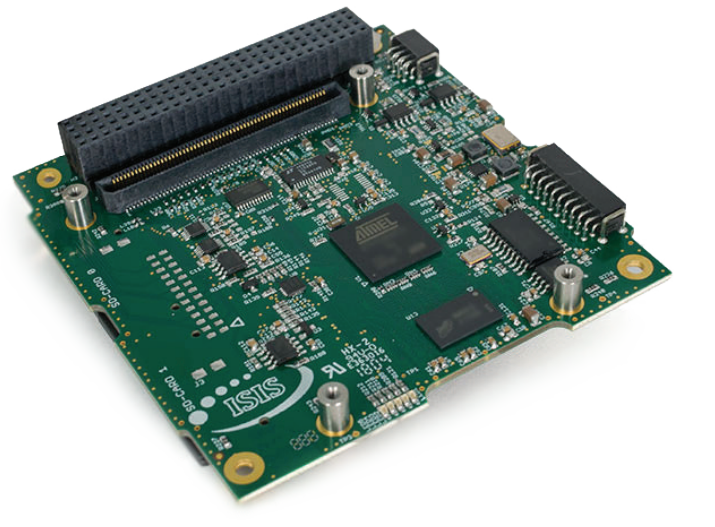
\includegraphics[keepaspectratio=true,scale=0.48]{figuras/isis.PNG}
	
	Fonte: Empresa ISIS\footnote{Empresa ISIS. 2018. Disponível em:\url{goo.gl/NfTdwS
		}. Acesso em: 31 maio 2018.}. \linebreak
	
	\label{fig14}
\end{figure}

\newpage
\item \textbf{FM430 Flight Module}

O FM430, da fabricante Pumpkin Inc, é uma solução compacta para sistemas ambientais difíceis. Possui como microcontrolador o MSP430F1612 de 16-bit, da fabricante Texas Instruments, com velocidade de clock de 7.3728 MHz. 50-60kB ROM e 2-10kB de RAM, 48 pinos I/O, 2 USART, 2 SPI, 1 I2C, 12-bit A/D e D/A, sensor de temperatura. SD Card para armazenamento (32MB – 2GB). Uma porta USB (Universal Serial Bus) e um conector de fonte de alimentação externa para facilitar a configuração pré-lançamento. A unidade do microcontrolador consome mais de 100 mW de potência (PUMPKIN,2008).

\begin{figure}[h]
	\centering
	\caption{Arquitetura do FM430.}
	
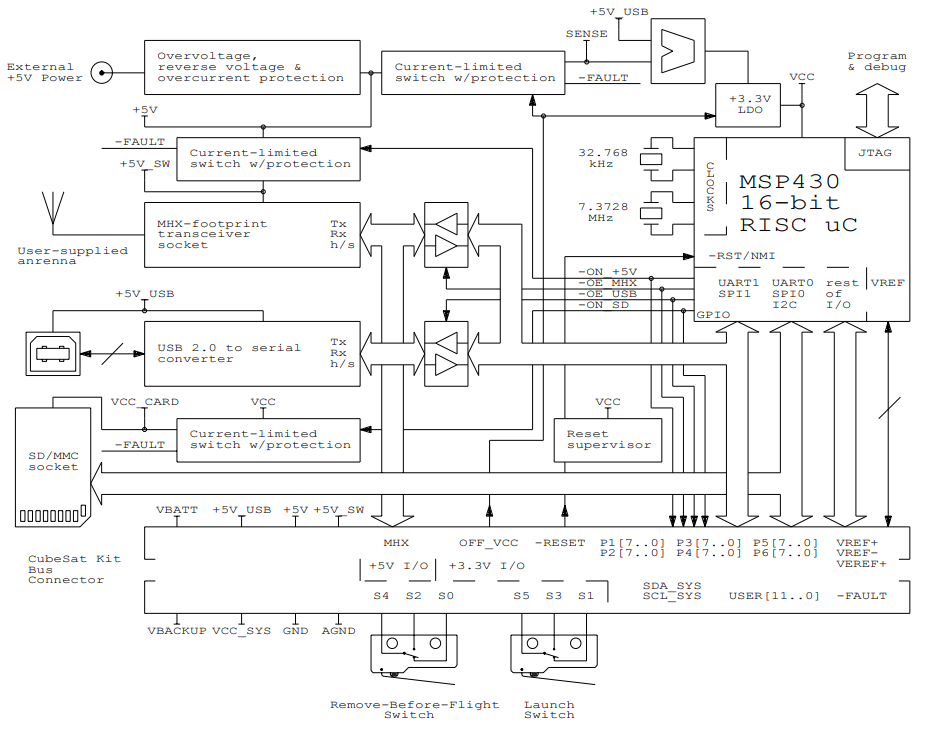
\includegraphics[keepaspectratio=true,scale=0.55]{figuras/fm430.PNG}
	
	Fonte:(PUMPKIN, 2008, pág.6).\linebreak
	\label{fig15}
\end{figure}

\end{itemize}

\newpage
\begin{itemize}
	\item \textbf{Tabela Comparativa entre os Computadores de Bordo}
	
	Abaixo há as características tabeladas.
	
	\begin{table}[h]
		\centering
		\caption{Tabela comparativa dos OBCs.}
		\label{tabela1}
		\makebox[1 \textwidth][c]{
			\scalebox{0.8}{
				\begin{tabular}{@{}c|cccc@{}}
					\hline
					\textbf{}      & \multicolumn{4}{c}{\textbf{Projetos}}                                          \\ \hline
					Projeto/OBC       & FloripaSat OBDH    & Open OBC          & iOBC              & FM430 Flight Mode \\
					Processador    & MSP430F6659IPZ     & TMS570LS0432      & AT91SAM9G20       & MSP430F1612       \\
					Fabricante     & Texas Instruments  & Texas Instruments & Micro Chip        & Texas Instruments \\
					Clock          & 8 MHz              & 80 MHz            & 400 MHz           & 7.3728 MHz        \\
					Watchdog Timer & Sim                & Sim               & Sim               & Sim               \\
					Memória Flash  & 512 KB             & 16 KB             & X                 & 55 KB             \\
					Memória RAM    & 66 KB              & 32 KB             & 32 KB             & 5 KB              \\
					EEPROM         & X                  & 16 KB             & X                 & X                 \\
					I2C            & 3                  & 0                 & 2                 & 1                 \\
					Canais ADC     & 16 canais de 12bit & 6 canais de 12bit & 6 canais de 10bit & 8 canais de 12bit \\
					CAN            & X                  & X                 & X                 & X                 \\
					SPI            & 3                  & 2                 & 2                 & 2                 \\
					PWM            & 5 canais           & 0                 & 6                 & 1                 \\
					UART           & 3                  & 1                 & 7                 & 2                 \\ \hline
		\end{tabular}}}
	\end{table}
	
\end{itemize}





\section{Padrão PC/104}

O PC/104 é o padrão de placas eletrônicas mais utilizado na indústria e em missões CubeSat. O PC/104 Embedded Consortium (2008) definiu as restrições mecânicas e elétricas para uma placa padrão de circuito impresso. As principais restrições podem ser encontradas a seguir:

\begin{itemize}
\item Cada placa deve ter uma forma de 90x96mm;
\item A potência por módulo deve estar entre 1-2W, limitando a corrente do barramento para 4mA.
\item Os módulos devem ser de 8-bits ou 18-bits, correspondendo ao barramento PC e PC/AT, respectivamente;
\item O espaçamento entre as placas não deve exceder 15,24mm;
\item Os conectores do barramento podem ser do tipo “empilhado” ou “não-empilhado” dependendo do projeto;
\item A altura dos componentes não deve exceder 11,05mm;
\item A uso do barramento deve estar de acordo com a a Tabela 2:\textit{8-bit and 16-bit ISA Bus Signal Assignments} do PC/104 Standard\footnote{PC/104 Standard, version 2.6. 2018. Disponível em:\url{https://pc104.org/wp-content/uploads/2015/02/PC104_Spec_v2_6.pdf}. Acesso em: 03 julho 2018.}.

\end{itemize}

A tecnologia PC/104 é vantajosa para missões CubeSat devido a padronização de dimensões, barramentos, interfaces mecânicas e elétricas. Esses fatores acarretam na redução de custos, riscos e tempo envolvidos no projeto, sem contar na versatilidade de integrar outras soluções presentes no mercado, que utilizam o mesmo padrão (JANES,2006). A Figura \ref{fig16} mostra as dimensões mecânicas para uma placa PC/104 de 8-bits. 

\begin{figure}[h]
	\centering
    \caption{ PCB Padrão PC104 8-bits.}
    
	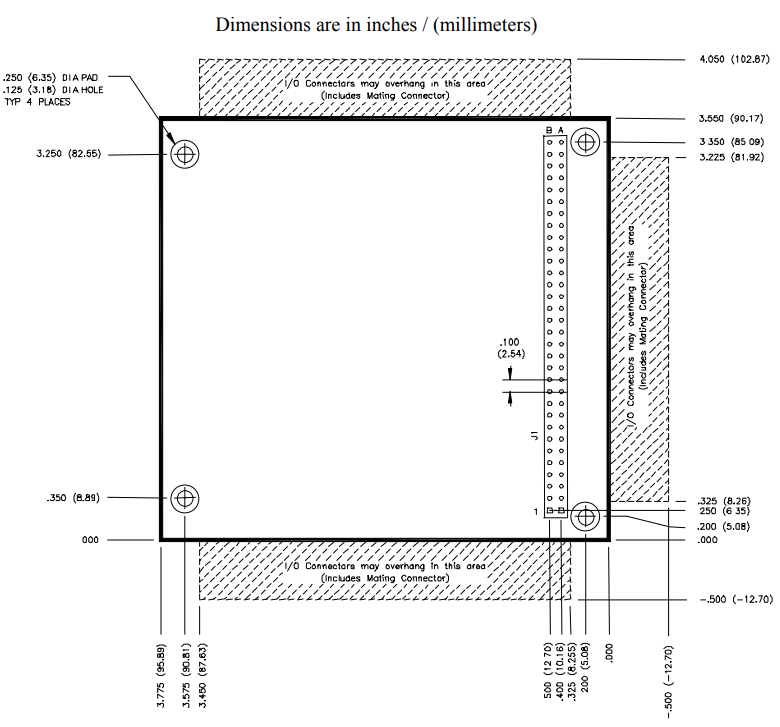
\includegraphics[keepaspectratio=true,scale=0.55]{figuras/pc104.PNG}
	
	Fonte: (PC/104 Embedded Consortium, 2008, pág.15).\linebreak
	\label{fig16}
\end{figure}

\section{Ambiente Espacial}
Um problema a ser considerado no desenvolvimento de um de um satélite, é o efeito do ambiente espacial nos subsistemas. Os problemas podem variar entre mal funcionamento operacional até danos físicos. Geralmente essas considerações são feitas para missões LEO (do inglês \textit{Low Earth Orbit}) e Deep Space (do inglês \textit{Espaço Profundo}) de longa duração (FROST; AGASID, 2015).

De acordo com Finckenor e Groh (2015), vários testes foram realizados na ISS (o inglês \textit{International Space Station}) para estudar a degradação dos materiais no ambiente espacial. Os principais efeitos são o vácuo, radiação ultravioleta, radiação espacial, plasma, temperaturas extremas, fadiga térmica e impacto de lixo espacial. 

Dentre os efeitos citados acima, o mais importante, para projetos da eletrônica embarcada é a radiação espacial (FROST; AGASID, 2015). Uma breve introdução sobre o tema e os possíveis efeitos no sistema embarcado será dado nas seções a seguir.

\subsection{Radiação Espacial}

A radiação no espaço é formada por partículas emitidas de várias fontes, dentro e fora do sistema solar. Os raios cósmicos (radiações primárias) interagem com gases e outras substâncias em altas altitudes, produzindo a radiação secundária. A combinação das radiações primárias e secundárias formam o ambiente de radiação espacial. As partículas desse ambiente podem causar degradação e falha dos sistemas embarcados (NASAa, 1996).

A quantidade de radiação que incide nos satélites depende da altitude e do tipo de órbita. A maioria dos CubeSats é colocado em órbitas LEO (altitude entre 100-1.000 km), recebendo uma dose de radiação de aproximadamente 0,1 krad/ano. Em missões com duração típica de 3-5 anos, a dose de radiação é menor que 0,5 krad/ano  (PETKOV, 2003).

De acordo com Petkov (2003), os efeitos provocados por essas radiações podem ser classificados de acordo com a Figura \ref{fig17}.

\begin{figure}[h]
	\centering
	
	\caption{Classificação dos efeitos da Radiação Espacial.}
	
	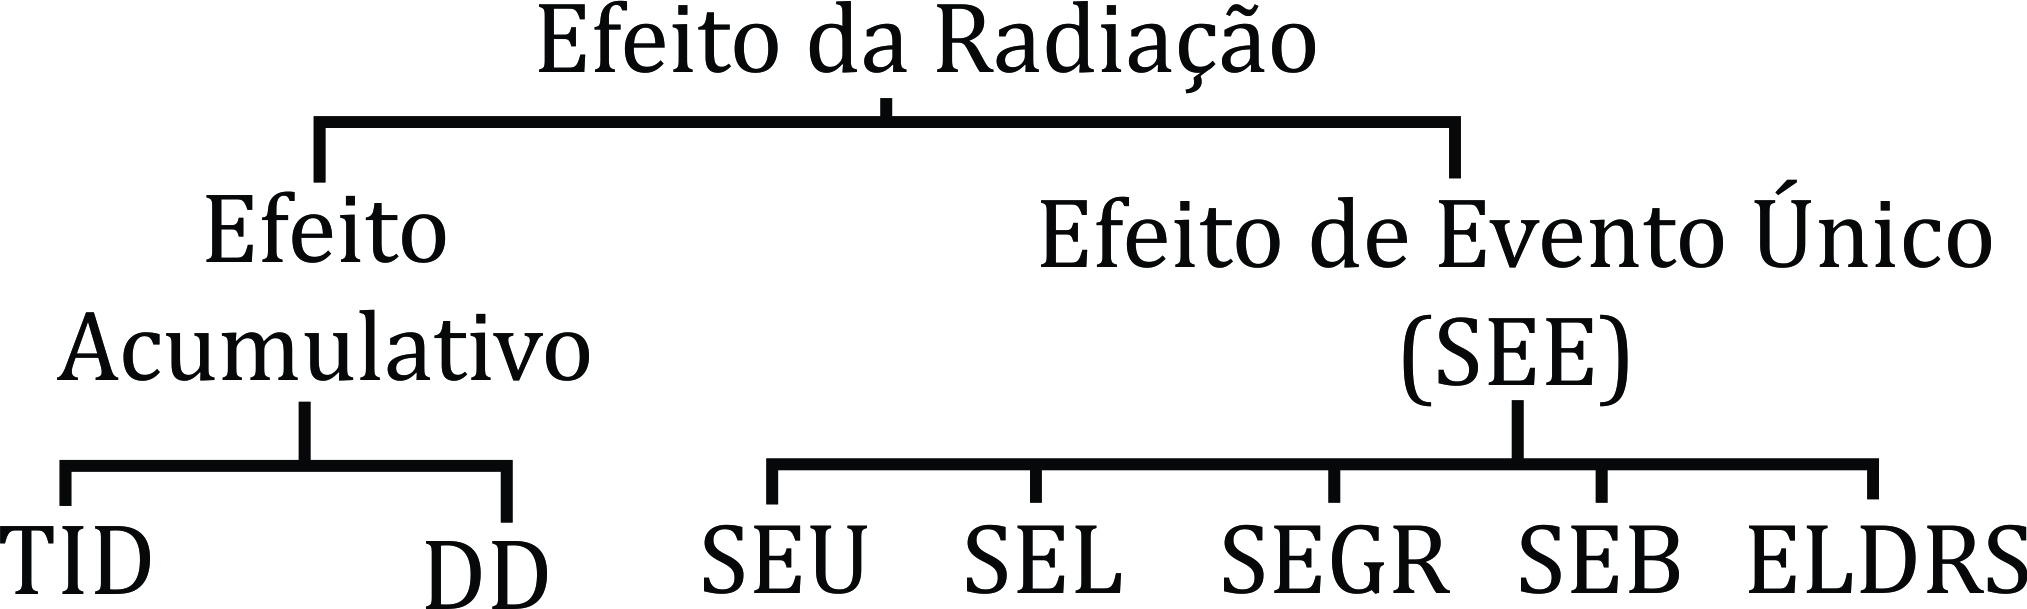
\includegraphics[keepaspectratio=true,scale=0.55]{figuras/radiation.jpg}
	
	\label{fig17}
\end{figure}

\begin{itemize}
\item \textbf{Efeito Acumulativo}

O Total de Dose Ionizante (TID, do inglês \textit{Total Ionizing Dose}) e o Dano de Deslocamento (DD, do inglês \textit{Displacement Damage}) são efeitos permanentes causados pela radiação ao longo do tempo. Com isso, o tempo da missão é um fator que intensifica tais efeitos. Abaixo há uma breve descrição sobre tais efeitos (PETKOV, 2003).

\begin{table}[h]
\centering
\caption{Efeitos Acumulativos causada pela radiação espacial.}
\label{tabela2}
\makebox[1 \textwidth][c]{
\scalebox{0.9}{
\begin{tabular}{@{}ll@{}}
\toprule
\multicolumn{1}{c}{\textbf{Efeito}} & \multicolumn{1}{c}{\textbf{Descrição}}                                                                                                                                    \\ \midrule
Total Ionizing Dose (TID)           & \begin{tabular}[c]{@{}l@{}}Incidência de radiação sobre o material. Ao longo do \\ tempo ocasiona mudança nas características elétricas, \\ levando à falhas\end{tabular} \\
Displacement Damage (DD)            & \begin{tabular}[c]{@{}l@{}}Deslocamento dos átomos em semicondutores, levando à \\ alteração das características elétricas do dispositivo\end{tabular}                    \\ \bottomrule
\end{tabular}}}
\end{table}


\item \textbf{ Efeito de Evento Único}

Efeitos de Evento Único (SEE, do inglês Single Event Effect) são efeitos ocorridos em dispositivos eletrônicos devido a passagem de uma única partícula pelo sistema. Essa passagem pode mudar um elemento bi estável ou estado digital de uma memória, acarretando em efeitos temporários e permanentes (PETKOV, 2003).

\begin{table}[h]
\centering
\caption{Efeitos de Evento Único causados pela radiação espacial.}
\label{tabela2}
\makebox[1 \textwidth][c]{
\scalebox{0.8}{
\begin{tabular}{@{}cl@{}}
\toprule
\multicolumn{1}{c}{\textbf{Efeito}}        & \multicolumn{1}{c}{\textbf{Descrição}}                                                                                              \\ \midrule
Single Event Upset (SEU)                   & Alteração temporária do estado do latch ou da memória                                                                               \\
Single Event Latchup (SEL)                 & \begin{tabular}[c]{@{}l@{}}Falha permanente causada pela quantidade de corrente \\ drenada durante o estado de latchup\end{tabular} \\
Single Event Gate Rupture (SEGR)           & \begin{tabular}[c]{@{}l@{}}Falha permanente do dispositivo, mais comum em \\ transistores de potência\end{tabular}                  \\
Single Event Burnout (SEB)                 & \begin{tabular}[c]{@{}l@{}}Falha permanente do dispositivo, mais comum em \\ transistores de potência\end{tabular}                  \\
Enhanced Low Dose Rate Sensitivity (ELDRS) & \begin{tabular}[c]{@{}l@{}}Falha permanente do dispositivo causada pela \\ radiação em baixas doses\end{tabular}                    \\ \bottomrule
\end{tabular}}}
\end{table}

\end{itemize}

\subsection{Categoria de Componentes}

A resistência a radiação dos componentes é um fator muito importante para estimar a taxa de falha e a vida útil do sistema. Há três categorias que os componentes eletrônicos podem se enquadrar, em relação a resistência a radiação: \textit{Comercial} (COTS), \textit{Rad Tolerant} e \textit{Rad-Hard}. Abaixo há uma breve descrição de cada uma, juntamente com os níveis de TID, SEU e taxa de SEU (NASA, 1999).

\begin{itemize}
\item \textit{Comercial}:
	
    \begin{itemize}
    \item O processo de design não garante resistência à radiação.
	\item Pouco controle da radiação.
	\item Níveis de resistência: 
    	
        \begin{itemize}
        \item Dose Total: 2 a 10 krad (típico).
		\item Limite de SEU: 5$\frac{MeV}{mg.cm^{2}}$.
		\item Taxa de erro SEU: $10^{-5}\frac{erros}{bit.dia}$ (típico).
        \end{itemize}
	\item O cliente realiza testes de radiação e assume todos os riscos.
	\item Avaliação e risco do cliente.

    \end{itemize}
    
\item \textit{Rad Tolerant:}
	\begin{itemize}
	\item O design garante resistência à radiação até um certo nível.
	\item Pouco controle da radiação.
	\item Níveis de resistência: 
		\begin{itemize}
		\item Dose Total: 20 a 50 krad (típico).
        \item Limite de SEU: 20 $\frac{MeV}{mg.cm^{2}}$.
		\item Taxa de erro SEU: ${10^{-7}}$-$10^{-8}\frac{erros}{bit.dia}$.
		\end{itemize}  

	\item Geralmente testado apenas para falha funcional.
    \item Avaliação e risco do cliente.

	\end{itemize}

\item \textit{Rad-Hard:}
	\begin{itemize}
	\item Projetado e processado para um nível de dureza específico
	\item Vários testes realizados com o substrato do chip
	\item Níveis de resistência: 
		\begin{itemize}
		\item Dose Total: > 200 krad a >1 Mrad.
        \item Limite de SEU: 80-150$\frac{MeV}{mg.cm^{2}}$.
		\item Taxa de erro SEU:${10^{-10}}$-$10^{-12}\frac{erros}{bit.dia}$.
		\end{itemize}  

	\item Geralmente testado apenas para falha funcional.
    \item Avaliação e risco do cliente.

	\end{itemize}
\end{itemize}


\chapter[DESENVOLVIMENTO DO HARDWARE]{DESENVOLVIMENTO DO HARDWARE}
\label{secaoHardware}
Esse capítulo descreverá o desenvolvimento do \textit{hardware}. Inicialmente será mostrado os requisitos e funcionalidades consideradas para o sistema. O passo seguinte é um dos mais importantes pois mostrará o processo de seleção do microcontrolador, componente que afetará restante do projeto. Em seguida será exposto os componentes adicionais que formarão o OBC, como: memória, sensores, etc. Por fim, será apresentado o esquemático do OBC e o \textit{layout} da placa de circuito impresso. 

\section{Requisitos e Funcionalidades}
\label{seção1_1}
Para o desenvolvimento de qualquer projeto, a definição dos requisitos é essencial, pois essa etapa influenciará as demais fases e definirá as expectativas das partes interessadas. Até o presente momento, poucos requisitos foram delimitados, pois o projeto da missão CubeSat ainda está em fase de discussão. 

A abordagem utilizada para contornar essa situação foi adicionar requisitos de CubeSats já lançados à alguns requisitos já especificados para a missão. No Apêndice \ref{apendiceb} há uma explicação sobre essa abordagem. 

Com base no Apêndice \ref{apendiceb}, foi possível delimitar as funcionalidades para o \textit{hardware} do sistema. Esses requisitos podem ser vistos na Tabela \ref{tabela1}.

\begin{table}[h]
\centering
\caption{Requisitos do Hardware.}
\label{tabela1}
\makebox[1 \textwidth][c]{
\begin{tabular}{@{}cl@{}}
\toprule
Número do Requisito & \multicolumn{1}{c}{Descrição do Requisito}                                                                                                                                                                                                    \\ \midrule
OBC-H-R1            & \begin{tabular}[c]{@{}l@{}}OBC deve realizar a aquisição dos seguintes dados: Temperatura;\\ Tensão e Corrente consumidas pelo sistema; Sensor Inercial;Dados \\dos demais subsistemas do CubeSat; Payload  (Imagens da Câmera).\end{tabular} \\ \hline
OBC-H-R2            & Possuir sistema de proteção contra travamentos.                                                                                                                                                                                               \\ \hline
OBC-H-R3            & \begin{tabular}[c]{@{}l@{}}Os componentes devem suportar a faixa de temperatura das \\órbitas baixas e heliossíncrona.\end{tabular}                                                                                                                                                                                               \\ \hline
OBC-H-R4            &\begin{tabular}[c]{@{}l@{}} O OBC deve possuir interfaces condizente com cada\\ subsistema do satélite.\end{tabular}                                                              \\ \hline
OBC-H-R5            & Possuir concepção versátil.                                                                                                                                                                                                                   \\ \hline
OBC-H-R6            & Possuir soluções que protejam o sistema contra falhas.                                                                                                                                                                                        \\ \hline
OBC-H-R7            & Possuir armazenamento não volátil de dados.                                                                                                                                                                                                   \\ \bottomrule
\end{tabular}}
\end{table}

\section{Análise do Microcontrolador}

O microcontrolador é um dos componente mais importante do OBC, pois ele executará o \textit{software} destinado ao gerenciamento do satélite. No processo de seleção do microcontrolador, utilizou-se as seguintes características como parâmetro de escolha:

\begin{itemize}
\item \textbf{Baixo Consumo:}
A energia disponível em um Cubesat depende da área de cobertura e eficiência dos painéis solares. De acordo com  Wiley J. e Richard Wertz (1992), os painéis solares podem fornecer, aproximadamente, 100W/m$^2$. Supondo que a futura missão tenha painéis solares fixados na superfície da plataforma 3U, um lado do CubeSat teria 0,03m$^2$ (3W) de cobertura. Supondo também que essa potência seja dividida igualmente entre os subsistemas (TT\&C, AODCS, OBC, EPS e PAYLOAD), o OBC teria disponível até 0,6W.

\item \textbf{Conversores AD:}
O OBC contará com muitos sensores (corrente, luminosidade, etc), sendo assim, conversores AD são importante para aferir os dados dos sensores. 

\item \textbf{Portas I/O:}
Possuir GPIO (do inglês \textit{General-Purpose Input/Output}) se torna importante para a comunicação com outros subsistemas do satélite. 

\item \textbf{Interfaces Seriais (UART, I2C, SPI):}
Os protocolos seriais são os mais utilizados entre os protocolos de comunicação digital. Com isso, possuir pinos dedicados à esses protocolos ajuda no desenvolvimento do OBC.

\item \textbf{PWM:}
Para o controle de atitude será necessário utilizar motores de passo, consequentemente há a necessidade de pinos que gerem sinais PWM.

\item \textbf{Frequência de Operação:}
Em aplicações embarcadas, a performance do microcontrolador é normalmente proporcional à frequência do clock.

\item \textbf{Faixa de Temperatura:}
Segundo CZERNIK (2004), a estimativa de temperatura em uma órbita LEO pode variar de -80$^{\circ}$C (eclipse), e 53$^{\circ}$C (insolação). Já para órbitas Sun-Síncronas, a estimativa de variação é de -27$^{\circ}$C à 43$^{\circ}$C (FRIEDEL, Jonas; MCKIBBON, Sean, 2011). O microcontrolador deverá suportar essas temperaturas.
\end{itemize}

A partir das características acima, procurou-se por microcontroladores das fabricantes mais usuais, como a Microchip e Texas Instruments. Optou-se pela seleção de microcontroladores que possuíssem uma placa de desenvolvimento, para viabilizar o tempo de implementação. Os dispositivos utilizados na escolha são expostos na Tabela \ref{tabela5}.

\newpage

% Please add the following required packages to your document preamble:
% \usepackage{booktabs}
\begin{table}[h]
\centering
\caption{Microcontroladores selecionados.}
\label{tabela5}
\makebox[1 \textwidth][c]{
\scalebox{0.8}{
\begin{tabular}{@{}ccccccccc@{}}
\toprule
Microcontrolador & Consumo                                                   & AD    & I/O & InterfaceSerial                                                   & PMW & \begin{tabular}[c]{@{}c@{}}Watchdog \\ Timer\end{tabular} & Frequência & \begin{tabular}[c]{@{}c@{}}Faixa de \\ Temperatura {[}$^{\circ}${C]}\end{tabular} \\ \midrule
MSP432P4111      & \begin{tabular}[c]{@{}c@{}}25mW \\ @ 48MHz\end{tabular}   & 24 AD & 84  & \begin{tabular}[c]{@{}c@{}}4 UART/SPI,\\ 4 I2C\end{tabular}       & Sim & sim                                                       & 48MHz      & -40 a 85                                                                         \\
MC9S12XHZ512     & \begin{tabular}[c]{@{}c@{}}30,9mW \\ @40MHz\end{tabular}  & 16 AD & 57  & \begin{tabular}[c]{@{}c@{}}3 UART/2 SPI,\\ 1 I2C\end{tabular}     & sim & sim                                                       & 40MHz      & -40 to 105                                                                       \\
MSP430F5529      & \begin{tabular}[c]{@{}c@{}}30,3mW \\ @ 25MHz\end{tabular} & 12 AD & 63  & \begin{tabular}[c]{@{}c@{}}2 UART/2 SPI,\\ 1 I2C\end{tabular}     & sim & sim                                                       & 25MHz      & -40 a 85                                                                         \\
RM42L432         & \begin{tabular}[c]{@{}c@{}}480mW \\ @ 100MHz\end{tabular} & 16 AD & 45  & \begin{tabular}[c]{@{}c@{}}2 UART/1 SPI,\\ 2 I2C\end{tabular}     & sim & sim                                                       & 100MHz     & -40 to 105                                                                       \\
ATSAMD21J18      & \begin{tabular}[c]{@{}c@{}}5mW \\ @ 48MHz\end{tabular}    & 20 AD & 52  & 6 UART/SPI/I2C                                                    & sim & sim                                                       & 48MHz      & -40 a 85                                                                         \\
ADuCM360         & \begin{tabular}[c]{@{}c@{}}18,15mW \\ @16MHz\end{tabular} & 4 AD  & 19  & \begin{tabular}[c]{@{}c@{}}1 UART, \\ 1 SPI,\\ 2 I2C\end{tabular} & sim & sim                                                       & 16MHz      & -40 a 125                                                                        \\ \bottomrule
\end{tabular}}}
\end{table}

Após a seleção dos microcontroladores, foi colocado pesos para cada característica de acordo com a importância no sistema. Vale a pensa ressaltar que os dados acima foram retirados dos \textit{datasheet} de cada microcontrolador. 


\begin{table}[h]
\centering
\caption{Pontuação de cada microcontrolador.}
\label{tabela3}
\makebox[1 \textwidth][c]{
\scalebox{0.8}{
\begin{tabular}{@{}cccccccccc@{}}
\toprule
Microcontrolador & Consumo & AD  & I/O  & Interface Serial & PMW & \begin{tabular}[c]{@{}c@{}}Watchdog \\ Timer\end{tabular} & Frequência & \begin{tabular}[c]{@{}c@{}}Faixa de \\ Temperatura {[}$^{\circ}${C]}\end{tabular} & SOMA  \\ \midrule
PESO             & 5       & 3   & 3    & 4               & 3   & 3                                                         & 5          & 4                                                                                & 30    \\ \midrule
MSP432P4111      & 5       & 3   & 3    & 3,5             & 3   & 3                                                         & 2,4        & 3,03                                                                             & 25,93 \\
MC9S12XHZ512     & 2,83    & 2   & 2,04 & 3,7             & 3   & 3                                                         & 2          & 3,52                                                                             & 22,09 \\
MSP430F5529      & 1,8     & 1,5 & 2,25 & 3               & 3   & 3                                                         & 1,25       & 3,03                                                                             & 18,83 \\
RM42L432         & 0,46    & 2   & 1,61 & 3,7             & 3   & 3                                                         & 5          & 3,52                                                                             & 22,29 \\
ATSAMD21J18      & 5       & 2,5 & 1,86 & 4               & 3   & 3                                                         & 2,4        & 3,03                                                                             & 24,79 \\
ADuCM360         & 1,93    & 0,5 & 0,68 & 3,5             & 3   & 3                                                         & 0,8        & 4                                                                                & 17,41 \\ \bottomrule
\end{tabular}}}
\end{table}

A partir da tabela acima pode-se observar que microcontroladores MSP432P4111 e o ATSAMD21J18 possuem as maiores nota. Ambos contam com processadores da família ARM Cortex M, sendo o Microchip da categoria M0+ e o TI da categoria M4F. Alguns pontos podem ser levantados em comparação aos dois microcontroladores:

\begin{itemize}
\item O microcontrolador da Texas Instruments possui 32 GPIOs e 4 ADC a mais que o microcontrolador da Microchip.

\item De acordo com a Figura \ref{fig18}, o MSP432P4111 (M4F) possui uma performance superior ao ATSAMD21J18 (M0+), aproximadamente 37\%.

\item Outro item que não foi colocado na tabela de comparação é a memória SRAM. O MSP432P4111 conta com 64 KB de SRAM contra 32 KB do ATSAMD21J18.

\end{itemize}


\begin{figure}[h]

    \centering
    \caption{ Performance dos processadores CORTEX-M.}
	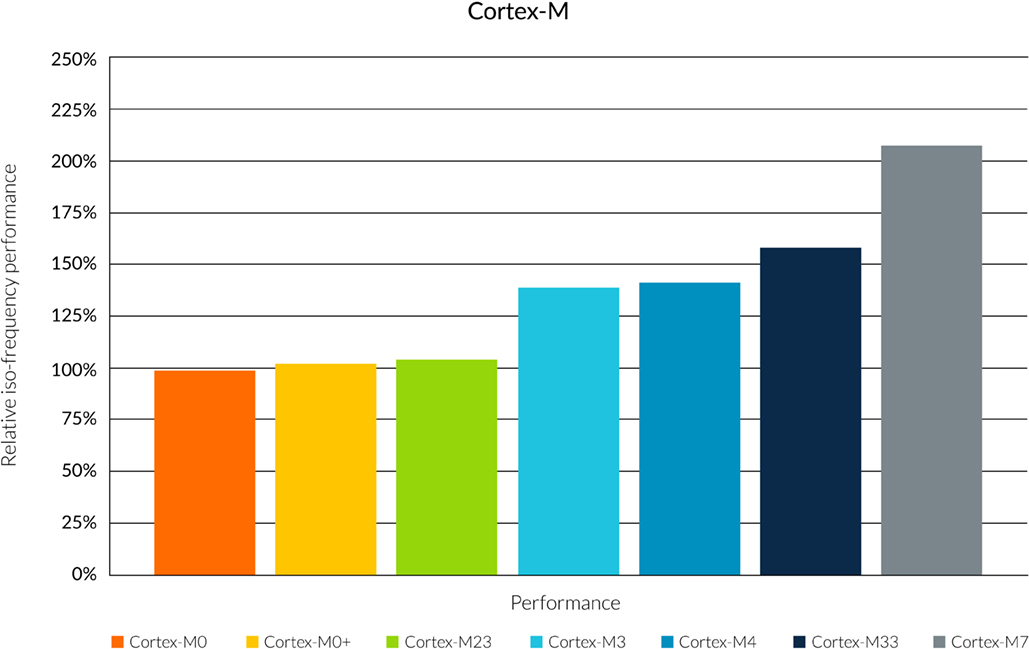
\includegraphics[keepaspectratio=true,scale=0.4]{figuras/arm-cortex-m-series-performance-graph.jpg}
	
	Fonte:(ARM Microcontrollers, 2018, pág.1).
	
	\label{fig18}
\end{figure}

A partir da análise acima, pode-se concluir que o MSP432P4111 é a melhor opção entre os microcontroladores analisados. Ele pode ser considerado uma ótima ferramenta em aplicações de baixo consumo, missões 1U, ou aplicações que há a necessidade de uma boa performance, missões 2U e 3U. Sendo assim o microcontrolador selecionado para o OBC é o MSP432P4111.

\section{Microcontrolador MSP432P4111}

As características do MSP432P4111 serão apresentadas nessa seção. Será mostrado o processador, unidade de memória interna, periféricos e consumo de energia em cada modo de operação. As referências utilizadas para essa seção foram o DataSheet do microcontrolador (Texas Instruments, 2018) e o livro Microcontroller Engineering with MSP432 (BAI, 2016). A Figura \ref{fig19} mostra o diagrama de blocos do MSP432P4111.

\begin{figure}[h]
	\centering
    \caption{Arquitetura do microcontrolador MSP432P4111.}
    
	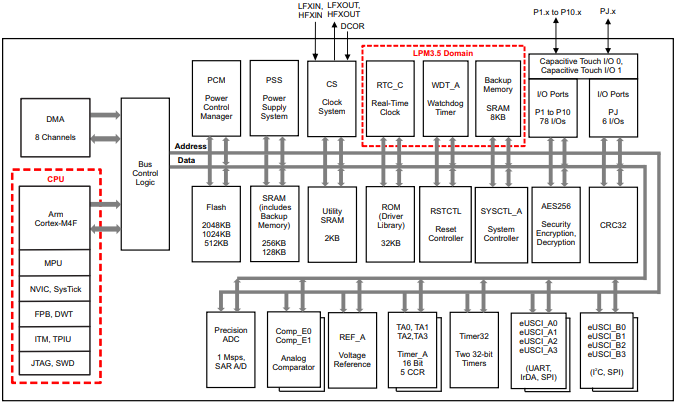
\includegraphics[keepaspectratio=true,scale=0.8]{figuras/msp432.PNG}
	
	Fonte: (Texas Instruments, 2018, pág.3).
	\label{fig19}
\end{figure}

O MSP432P4111 possui como microprocessador o ARM Cortex-M4F. Esse microprocessador possui arquitetura \textit{Reduced Instruction Set Computing} (RISC) com  32-bit de instrução, podendo operar em frequências acima de 48MHz. Ele foi projetado para aplicações que exigem baixa potência, alta eficiência, boa capacidade de processamento de sinais, baixo custo e fácil usabilidade. Esse microcontrolador não possui nenhuma unidade de armazenamento, entretanto, ele oferece interfaces para memórias ROM e SRAM externas. Devido ao tamanho de instrução, 32-bit, a capacidade máxima pesquisável para a memória é de 4GB, podendo haver mais de uma unidade de armazenamento com esse tamanho (Texas Instruments, 2018).

O barramento interno é de 32-bit, também chamado de \textit{Advanced Microcontroller Bus Architecture} (AMBA). Esse tipo de barramento oferece eficiência de operação e baixo consumo. O barramento principal entre o MCU e os componentes externos é o \textit{Advanced High Performance Bus} (AHB), oferecendo interface com a memória e os periféricos (BAI, 2018).

Mesmo o microprocessador possuindo o \textit{System Control Block}, que informa se houve algum erro na operação do sistema, não é tolerante à falhas. 

\subsection{Unidade de Memória}

O MSP432P4111 possui os seguintes componentes de memória:

\begin{itemize}
\item 2048KB Memoria Flash principal;
\item 32KB Memória Flash de informação (área utilizada para \textit{Bootloader, TVL} e \textit{Flash MailBox});
\item 256KB SRAM (incluindo 8KB de memória de backup);
\item 32KB ROM carregada com as bibliotecas MSP432™ \textit{Peripheral Driver}.
\end{itemize}

Esse microcontrolador suporta um endereçamento de 4GB dividido em oito zonas de 512MB. A memória de 2048KB serve para armazenar o programa do usuário.

\subsection{Portas e Periféricos}

O microcontrolador MSP432P4111 possui 11 	portas de propósito geral (GPIO), cada porta pode variar de 1 a 10. Para o controle de saída e entrada utiliza-se os registradores: PxIN, PxOUT, PxDIR, PxREN e PxDS. Para selecionar as portas, utiliza-se os registradores: PxSEL0, PxSEL1 e PxSEL2. Por fim, para configurar as interrupções das portas, utiliza-se os registradores: PxIFG, PxIES, PxIE e PxIV. O valor de ‘x’ indica o número da porta, 1 a 10 (BAI, 2018).

O microcontrolador conta com os seguintes periféricos:

\begin{itemize}
\item 4 UART, com frequência de clock até 7 MHz;
\item 4 I2C, com frequência de clock até 1MHz;
\item 8 SPI;
\item 24 ADC canais de 14-bit;
\item 84 I/O;
\item 4 Temporizadores de 16-bit ( Captura, Comparação e PWM);
\end{itemize}

\subsection{Consumo e Modos de Operação}

O microcontrolador suporta alguns modos de operação que permitem otimizar a potência consumida pelo sistema a cada aplicação. O \textit{Power Control Manager} (PCM) é responsável por gerenciar os modos de baixo consumo de cada área do sistema. 
	
    No Apêndice \ref{apendicec} há uma tabela que mostra todos os modos de operação, com uma descrição e o consumo em cada modo.

\section{Unidade de Armazenamento}

Geralmente, em projetos de sistemas embarcados, após a escolha do microcontrolador é realizada a escolha da memória. Mesmo o microprocessador possuindo 2048KB de memória Flash e 256KB de SRAM, será implementado um banco de memória externo que será destinada ao armazenamento do dados de telemetria e da \textit{payload}.

Diante da grande variedade de memórias disponíveis, a escolha do tipo de memória para esta aplicação se tornou uma tarefa exaustiva. Nesse processo de escolha, foi utilizada uma tabela comparativa, presente no \textit{Small Spacecraft Technology State of the Art} (FROST; AGASID,2015) e ilustrada abaixo.


\begin{table}[h]
\centering
\caption{Comparação dos tipos de Memória.}
\label{tabela_memoria}
\makebox[1 \textwidth][c]{
\scalebox{0.7}{
\begin{tabular}{@{}ccccccc@{}}
\toprule
Característica                                                                     & SRAM                                                      & DRAM       & Flash                                                                                               & MRAM                                                      & FRAM                                                                    & CRAM/PCM                                                  \\ \midrule
Não-Volátil                                                                        & Não                                                       & Não        & Sim                                                                                                 & Sim                                                       & Sim                                                                     & Sim                                                       \\
\begin{tabular}[c]{@{}c@{}}Tensão de operação,\\ +- 10\%\end{tabular}            & 3.3 – 5 V                                                 & 3.3 V      & 3.3 e 5 V                                                                                           & 3.3 V                                                     & 3.3 V                                                                   & 3.3 V                                                     \\
\begin{tabular}[c]{@{}c@{}}Organização\\   bits/die\end{tabular}                   & 512k x 8                                                  & 16M x 8    & 16M x 8; 32M x 8                                                                                    & 128k x 8                                                  & 16k x 8                                                                 & -                                                         \\
\begin{tabular}[c]{@{}c@{}}Retenção\\   de Dados (@70$^{\circ}$ C)\end{tabular}              & N/A                                                       & N/A        & 10 anos                                                                                             & 10 anos                                                   & 10 anos                                                                 & 10 anos                                                   \\
\begin{tabular}[c]{@{}c@{}}Resistencia\\   (Ciclo de Deletar/Escrita)\end{tabular} & Ilimitado                                                 & Ilimitado  & 10$^6$                                                                               & 10$^13$                                    & 10$^13$                                                  & 10$^13$                                    \\
Tempo de Acesso                                                                    & 10 ns                                                     & 25 ns      & \begin{tabular}[c]{@{}c@{}}50 ns depois de uma \\ pagina lida;\end{tabular}                         & 300 ns                                                    & 300 ns                                                                  & 100 ns                                                    \\
\begin{tabular}[c]{@{}c@{}}200ms\\   escrita; 2ms para deletar\end{tabular}        &                                                           &            &                                                                                                     &                                                           &                                                                         &                                                           \\
\begin{tabular}[c]{@{}c@{}}Radiação\\   (TID)\end{tabular}                         & 1Mrad                                                     & 59krad     & 30krad                                                                                              & 1Mrad                                                     & 1 Mrad                                                                  & 1 Mrad                                                    \\
\begin{tabular}[c]{@{}c@{}}SEU\\   rate (relativo)\end{tabular}                    & zero                                                      & Alto       & \begin{tabular}[c]{@{}c@{}}zero (celulas); Baixo -Medio\\   (dispositivos eletronicos)\end{tabular} & zero                                                      & zero                                                                    & zero                                                      \\
\begin{tabular}[c]{@{}c@{}}Faixa de\\   Temperatura\end{tabular}                   & \begin{tabular}[c]{@{}c@{}}Padrão \\ Militar\end{tabular} & Industrial & Comercial                                                                                           & \begin{tabular}[c]{@{}c@{}}Padrão \\ Militar\end{tabular} & \begin{tabular}[c]{@{}c@{}}Padrão \\ Militar\end{tabular}               & \begin{tabular}[c]{@{}c@{}}Padrão \\ Militar\end{tabular} \\
Potência                                                                           & 500 mW                                                    & 300 mW     & 30 mW                                                                                               & 900 mW                                                    & 270 mW                                                                  & -                                                         \\
Pacote                                                                             & 4MB                                                       & 128 MB     & 128 – 256 MB                                                                                        & 1 MB                                                      & \begin{tabular}[c]{@{}c@{}}1.5 MB \\ (pacote com 12 chips)\end{tabular} &                                                           \\ \bottomrule
\end{tabular}}}
Fonte: (FROST; AGASID, 2015, pág.97).\linebreak
\end{table}

De acordo com a Tabela \ref{tabela_memoria}, as memória MRAM e FERAM (ou FRAM) são as que mais resistem a radiação (TID), o que as caracterizam como ótimas alternativas para a unidade de armazenamento. Comparando-se essas memórias, pôde-se observa-se que ambas possuem as seguintes características em comum: não-volatilidade, tensão de operação, retenção de dados, ciclos de operação, tempo de acesso, TID, SEU e  faixa de temperatura.

Dentre as características distintas entre as memórias MRAM e FRAM, observa-se que a memória do MRAM gasta três vezes mais energia que a memória do FRAM. Como o quesito consumo elétrico é primordial em aplicações espaciais, a memória FRAM foi escolhida para compor a unidade de armazenamento. Essa memória será destinada para arquivar o software embarcado.

Para escolher o tamanho da memória FRAM, há a necessidade de estimar o tamanho do software embarcado. Esse software depende de vários fatores, como: redundâncias, funcionalidades implementadas, segurança, algoritmos, etc, o que torna essa estimativa muito complicado. Sendo assim, definiu-se o espaço como o dobro da memória SRAM do microcontrolador,  resultando em 512KB.

Em relação ao espaço para a telemetria e dados dos subsistemas, foi realizado uma estimativa, utilizando os parâmetros de armazenamento de dados da missão \textit{SWISSCube}. Esses parâmetros foram adaptados ao contexto do projeto, adicionando os dados proveniente da Câmera. Esses parâmetros se encontram no Apêndice \ref{apendiced}.

A partir dessa estimativa, a quantidade de dados armazenado em 1 dia seria de 176MB, 10MB proveniente de telemetría e 166MB da \textit{Payload} (imagens). Desse modo, um cartão de 512MB seria mais que o suficiente para armazenar os dados provenientes do sistema em 2 dias. Entretanto, como não se sabe a quantidade de estações de solo disponíveis para descarregar os dados, optou-se por escolher o tamanho máximo que o microcontrolador pode suportar, que no caso é de 4GB.

A memória Flash é a única que possui uma arquitetura que comporta 4GB de capacidade. Com isso, foi selecionado um cartão de memória com 4GB de capacidade para armazenar os dados da telemetria e da \textit{Payload}. 

Para a escolha dos fornecedores, escolheu-se o site \textit{DigiKey}\footnote{Disponível em: \url{https://www.digikey.com}}. Esse site possui filtros que ajudaram na seleção dos itens. O preço foi o fator decisório na seleção. As memórias escolhidas e suas características são mostradas na Tabela \ref{meoriasEscolhidas}.

\begin{table}[h]
\centering
\caption{Especificação das memórias da Unidade de Armazenamento.}
\label{meoriasEscolhidas}
\makebox[1 \textwidth][c]{
\scalebox{0.74}{
\begin{tabular}{@{}ccccccc@{}}
\toprule
PRODUTO          & Fornecedor                        & Temp OP          & Corrente & Vin               & Capacidade      & Protocolo \\ \midrule
FM25V05-GTR      & Cypress Semiconductor Corporation & -40$^{\circ}$C $\sim$85$^{\circ}$C & 300uA    & 2 V $\sim$3.6 V   & 512Kb (64K x 8) & SPI       \\
SQF-MSDM1-4G-21E & Advantech Corp                    & -40$^{\circ}$C $\sim$85$^{\circ}$C & 150uA    & 2.7 V $\sim$3.6 V & 4GB             & SPI       \\ \bottomrule
\end{tabular}}}
\end{table}

\section{Periféricos}

	Essa seção visa mostrar os sensores utilizados para compor o sistema e ajudar o microcontrolador a atingir os requisitos exigidos na Seção \ref{seção1_1}.

\subsection{Sensor de Corrente}

Com o intuito de cumprir o requisito de leitura de corrente, escolheu-se o sensor ACS711. Esse sensor possui um diferencial, ele conta com um sistema que protege o circuito contra sobre corrente, em caso de panes elétricas e tempestades solares. O ACS711 suporta valores de 3 a 5V de tensão e -40 a 125$^{\circ}$C de temperatura.

A figura \ref{fig20} mostra o esquemático eletrônico de uma aplicação usual do ACS711.



\begin{figure}[h]
	\centering
    \caption{Esquemático Eletrônico de uma aplicação usual do ACS711.}
    
	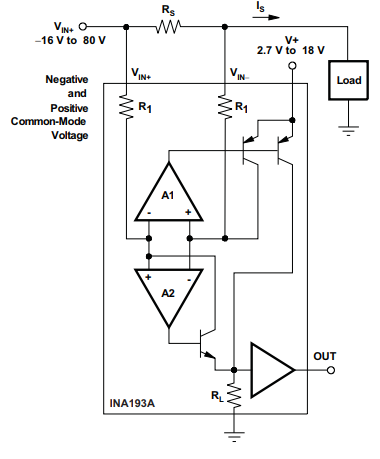
\includegraphics[keepaspectratio=true,scale=0.5]{figuras/currentSensor.PNG}
	
	Fonte:(ALLEGRO, 2017, pág.1)\linebreak
	
	\label{fig20}
\end{figure}

A tabela \ref{tab_ina} mostra as especificações do ACS711. Essas informações foram retiradas da ficha técnica do sensor.

\begin{table}[h]
\centering
\caption{Informações técnicas do ACS711.}
\label{tab_ina}
\makebox[1 \textwidth][c]{
\scalebox{0.74}{
\begin{tabular}{cccccc}
\hline
Produto    & Fornecedor        & \begin{tabular}[c]{@{}c@{}}Temp Op\\ {[}$^{\circ}$C{]}\end{tabular} & \begin{tabular}[c]{@{}c@{}}\textit{Overcurrent limit} \\ {[}A{]}\end{tabular} & \begin{tabular}[c]{@{}c@{}}Vin \\ {[}V{]}\end{tabular} & \begin{tabular}[c]{@{}c@{}}Erro\\ {[}\%{]}\end{tabular} \\ \hline
ACS711 & Allegro & -40$\sim$125                                                        & 100                                                        & 3$\sim$5                                           & 5                                                     \\ \hline
\end{tabular}}}
\end{table}

%\subsection{Sensor de Tensão}


\subsection{Sensor Inercial}

O sensor inercial será responsável por realizar as medidas inerciais nos 3 eixos, dados que possibilitará o controle das rodas de reação do AODCS. O MPU9250, fabricado pela \textit{TKD ENVISENSE}, foi escolhido para realizar essa tarefa. Esse sensor possui acelerômetro, magnetômetro e giroscópio nos 3 eixos, além de um sensor de temperatura (INVENSENSE, 2018).

A Tabela \ref{tab_ive} mostra as especificações do MPU9250. Essas informações foram retiradas da ficha técnica do sensor.

\begin{table}[h]
\centering
\caption{Informações técnicas sobre sensor MPU9250.}
\label{tab_ive}
\makebox[1 \textwidth][c]{
\scalebox{0.9}{
\begin{tabular}{@{}ccccccl@{}}
\toprule
Produto  & Fornecedor     & \begin{tabular}[c]{@{}c@{}}Temp. Op. \\ {[}$^{\circ}$C{]}\end{tabular} & \begin{tabular}[c]{@{}c@{}}Corrente \\ {[}mA{]}\end{tabular} & \begin{tabular}[c]{@{}c@{}}Vin \\ {[}V{]}\end{tabular} & Resolução {[}bit{]}                                                                         & Protocolo \\ \midrule
MPU-9250 & TDK InvenSense & -40 $\sim$85                                                           & 3.2mA                                                        & 2.4 $\sim$3.6                                          & \begin{tabular}[c]{@{}c@{}}Giro./Ace. -\textgreater 16\\ Mag. -\textgreater 14\end{tabular} & SPI/I2C   \\ \bottomrule
\end{tabular}}}
\end{table}

A figura \ref{mpu} mostra o esquemático eletrônico de uma aplicação usual do MPU9250, utilizando protocolo I2C(esquerda) e SPI (direita).

\begin{figure}[h]
	\centering
	\caption{Esquemático Eletrônico de uma aplicação usual do MPU9250.}
    
	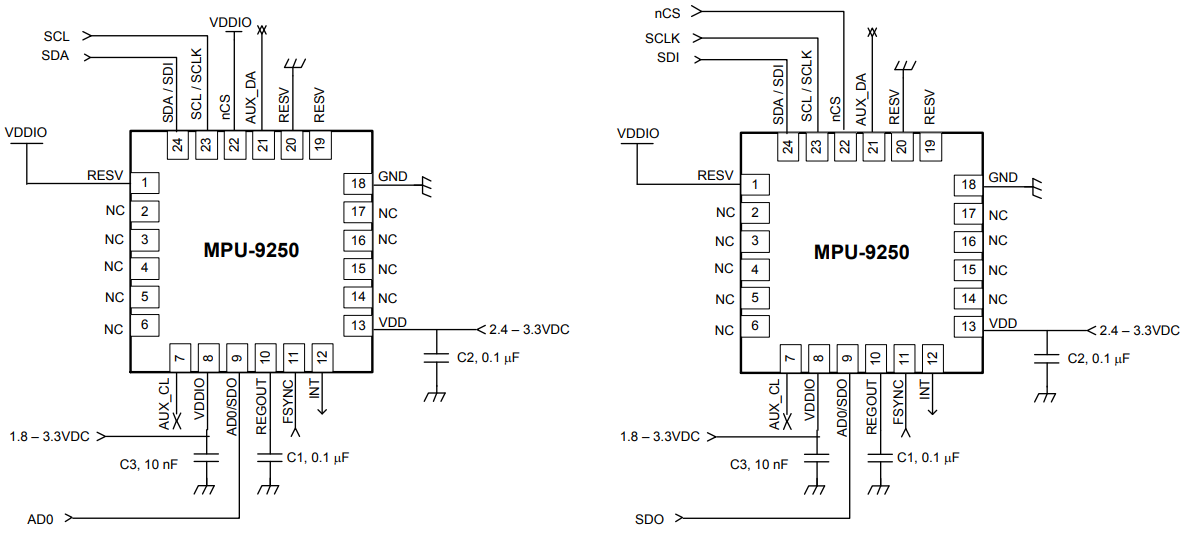
\includegraphics[keepaspectratio=true,scale=0.4]{figuras/mpu9250.PNG}
	
	Fonte:(INVENSENSE, 2018, pág.20)\linebreak
	
	\label{mpu}
\end{figure}

\subsection{Sensor de Temperatura}

Mesmo o MPU9250 e o MSP432P4111 possuindo um sensor de temperatura, foi escolhido outro para realizar a medida da temperatura do OBC. Possuir um sensor de temperatura dedicado à essa função é ideal, pois as funções primárias do MPU9250/MSP432P4111 podem interferir no valor das medidas. Por exemplo, o microcontrolador começará a esquentar após um período muito longo em modo de alta performance. 

O sensor de temperatura escolhido foi o MCP9701T, da fabricante Microchip, devido sua fácil usabilidade e baixo consumo. O dispositivo comunica através de uma saída analógica, sendo capaz de medir temperaturas com uma precisão de 2 $^{\circ}$C em uma faixa de temperatura de -40$^{\circ}$C a 125$^{\circ}$C (MICROCHIP, 2016).

A tabela \ref{caracTMP} mostra as especificações do MCP9701T. Essas informações foram retiradas da ficha técnica do sensor.
http://ww1.microchip.com/downloads/en/devicedoc/20001942g.pdf
\begin{figure}[h]
	\centering
	\caption{Esquemático Eletrônico de uma aplicação usual do MCP9700.}
	
	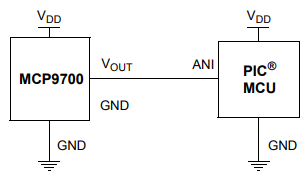
\includegraphics[keepaspectratio=true,scale=0.6]{figuras/MCP9700.PNG}
	
	Fonte:(MICROCHIP, 2018, pág.20)\linebreak
	\label{MCP9700}
\end{figure}

\begin{table}[h]
\centering
\caption{Informações técnicas sobre sensor MCP9701T.}
\label{caracTMP}
\begin{tabular}{@{}ccccccc@{}}
\toprule
Produto   & Fornecedor                                                   & \begin{tabular}[c]{@{}c@{}}Temp. Op. \\ {[}$^{\circ}$C{]}\end{tabular} & \begin{tabular}[c]{@{}c@{}}Corrente \\ {[}uA{]}\end{tabular} & \begin{tabular}[c]{@{}c@{}}Vin \\ {[}V{]}\end{tabular} & \begin{tabular}[c]{@{}c@{}}Resolução \\ {[}bit{]}\end{tabular} & Comunicação \\ \midrule
MCP9701T & \begin{tabular}[c]{@{}c@{}}Microchip\end{tabular} & -55 $\sim$127                                                          & 60                                                           & 2.7 $\sim$5.5                                          & 12                                                             & Analógico       \\ \bottomrule
\end{tabular}
\end{table}

\section{Interface de Programação/\textit{Debug}}

O MSP432P4111 possui dois tipos de interface de programação: JTAG (\textit{Joint Test Action Group}), SWD (\textit{Serial Wire Debug}). Essas duas interfaces são utilizadas em conjunto para programar e "\textit{debugar}" o microcontrolador\footnote{Disponível em: http://www.ti.com/lit/ug/slau747b/slau747b.pdf}. 

Os pinos destinados para a interface JTAG/SDW são mostrados na Tabela \ref{jtagPin}.

\begin{table}[h]
	\centering
	\caption{Pinos JTAG no MSP432P4111.}
	\label{jtagPin}
	\begin{tabular}{@{}ccc@{}}
		\toprule
		Sinal   & Descrição & Pino 
		\\ \midrule
		TCK\underline{ }SWCLK & JTAG clock input (TCK) & P.95
		\\ \midrule
		TMS\underline{ }SWDIO & JTAG test mode select (TMS) & P.94
		\\ \midrule
		TDO\underline{ }SWO & JTAG trace output (TWO) & P.93
		\\ \midrule
		TDI & JTAG test data input & P.92        
		\\ \bottomrule
	\end{tabular}
\end{table}


%\subsection{Barramento PC104}


\section{Dimensões da Placa}

Como foi mencionado anteriormente, o formato da placa seguirá o padrão \textit{PC/104-Plus}. Esse padrão é comumente visto em missões CubeSat. A placa possui dimensões físicas de 90.17 x 95.89 mm, possuindo 4 furos M3 nas extremidades da placa. A Figura \ref{pc104} ilustra as dimensões da placa estabelecida pelo \textit{PC/104 Consorsium}.

\begin{figure}[h]
	\centering
	\caption{Dimensões do módulo PC/104-Plus em polegadas e milímetros.}
	
	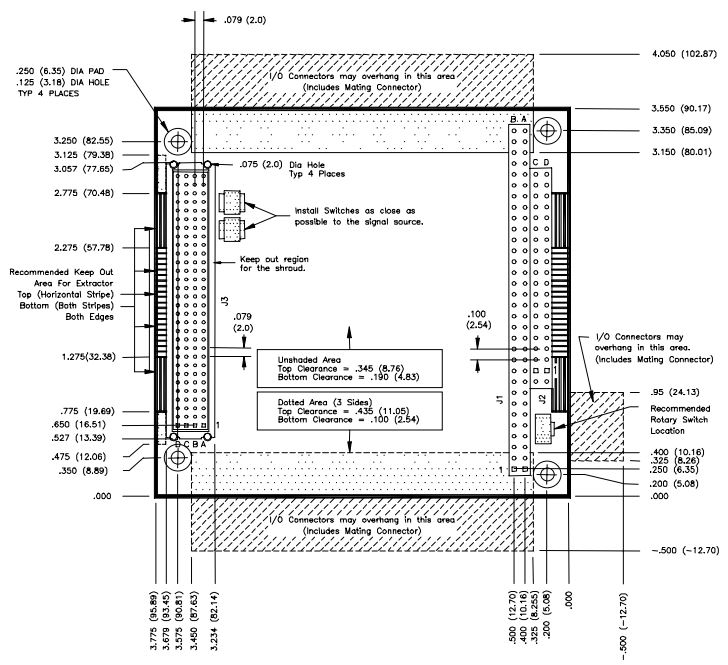
\includegraphics[keepaspectratio=true,scale=0.7]{figuras/pc104_32bit.PNG}
	
	Fonte:(PC/104 EMBEDDED CONSORTIUM, 2008, pág.20)
	
	\label{pc104}
\end{figure}

\section{Sistema para Mitigar Falhas}

De acordo com  Frost e Agasid (2015), missões de longa duração necessitam de mecanismos que diminuam o risco devido à radiação espacial. Como o microcontrolador e os componentes selecionados no projeto não possuem classificação \textit{Rad-Hard}, optou-se pela utilização de mecanismos que atenuassem as falhas. 

A partir de uma breve pesquisa, levantou-se as seguintes estratégias:
\begin{itemize}
	\item Proteção Metálica (EMI \textit{Shielding});
	\item Proteção contra corrente excessiva (\textit{OverCurrent});
	\item Código Corretor;
	\item \textit{Watchdog} externo.
\end{itemize}

Dentre as estrategias acima, a única que será discutida é a\textit{Watchdog} externo pois é uma solução simples e que não demanda muito tempo de implementação. As demais estrategias podem ser implementadas em uma segunda versão do computador de bordo.

\begin{comment}
	\subsection{Proteção contra corrente excessiva (\textit{OverCurrent})}
	
	Conforme mencionado anteriormente, o sensor de corrente ACS711 possui um sistema de proteção contra corrente excessiva. Isso se torna uma vantagem, pois caso ocorra alguma anomalia no EPS, ou qualquer outro sistema que afete o suprimento de energia, o OBC não será danificado.
	
	O funcionamento do ACS711, caso a corrente suba mais que o permitido
	
	Com o intuito de cumprir o requisito de leitura de corrente, escolheu-se o sensor ACS711. Esse sensor possui um diferencial, ele conta com um sistema que protege o circuito contra sobre corrente, em caso de panes elétricas e tempestades solares. O ACS711 suporta valores de 3 a 5V de tensão e -40 a 125$^{\circ}$C de temperatura.
	
	A figura \ref{fig20} mostra o esquemático eletrônico de uma aplicação usual do ACS711.
	
\end{comment}


\subsection{\textit{Watchdog} Externo}

Conforme  Frost e Agasid (2015), o \textit{Watchdog}  é normalmente utilizado para monitorar o estado do microcontrolador, evitando o travamento do sistema. Basicamente, um \textit{Watchdog} externo é um contador regressivo que, ao final da contagem, reinicia o microcontrolador em caso de um evento SEE. 

O microcontrolador já possui um \textit{Watchdog} interno que reiniciará o microcontrolador em caso de travamento. O uso de um contador externo trará mais robustez ao sistema.

O contador utilizado para o sistema de \textit{Watchdog} externo foi o STWD100, o mesmo utilizado pelo projeto do Botma (2011). Esse dispositivo é produzido pela fabricante STMicroelectronics e possui três tempos para \textit{reset} (3.4 ms, 6.3 ms, 102 ms e 1.6 s).  

A escolha do tempo de \textit{reset} será feita durante o teste do protótipo. Nessa fase, o \textit{software} embarcado estará com a logica de programação de todos os subsistemas estará finalizado, disponibilizando o tempo de execução de todas as \textit{Tasks}.

\newpage

\section{Placa de Circuito Impresso}


\begin{comment}

Apos a escolha dos componentes é possível ter uma visão abrangente do \textit{hardware}, como é mostrado na Figura \ref{arquiteturaOBC}. Como é possível notar, ha algumas interfaces que ainda nao foram definidas, como os pinos do modulo \textit{PPT} e \textit{TTC}.


\begin{figure}[h]
\centering
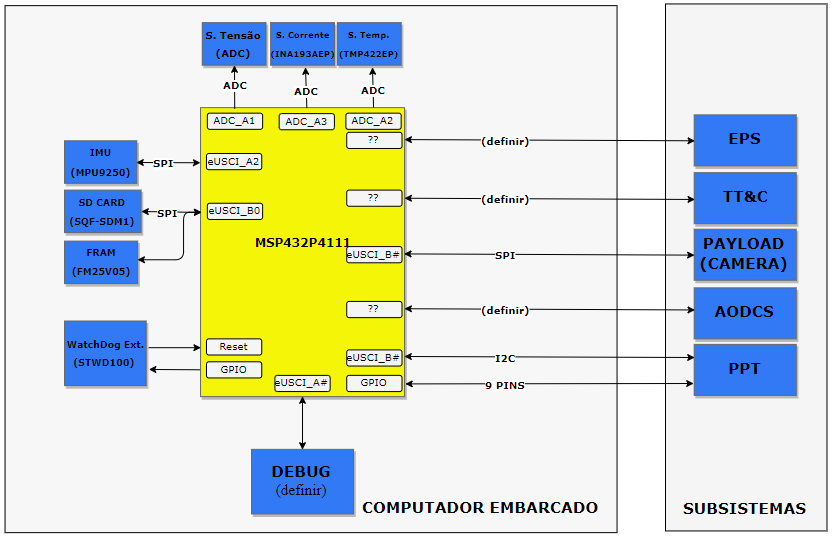
\includegraphics[keepaspectratio=true,scale=0.78]{figuras/arquiteturaHard2.PNG}
\caption{Arquitetura do OBC.}
\label{arquiteturaOBC}
\end{figure}

\end{comment}

Para o elaboração da placa de circuito impresso utilizou-se o software KiCad\footnote{Para mais detalhes, consulte:  http://www.kicad-pcb.org/}. Essa ferramenta possui uma interface amigável e fácil de usar, sendo bem difundida na comunidade de engenharia eletrônica e \textit{hobistas}. O fato do KiCad ser \textit{Open Source} facilita a manutenção do OBC em futuras melhorias, pois não ha a necessidade de comprar uma licença.

A Figura \ref{esquematicoObc} mostra o esquemático eletrônico do OBC. Nele há todos os competentes/sensores mencionados anteriormente. Foi utilizado o \textit{datasheet} de cada sensor para o desenvolvimento do esquemático. 

%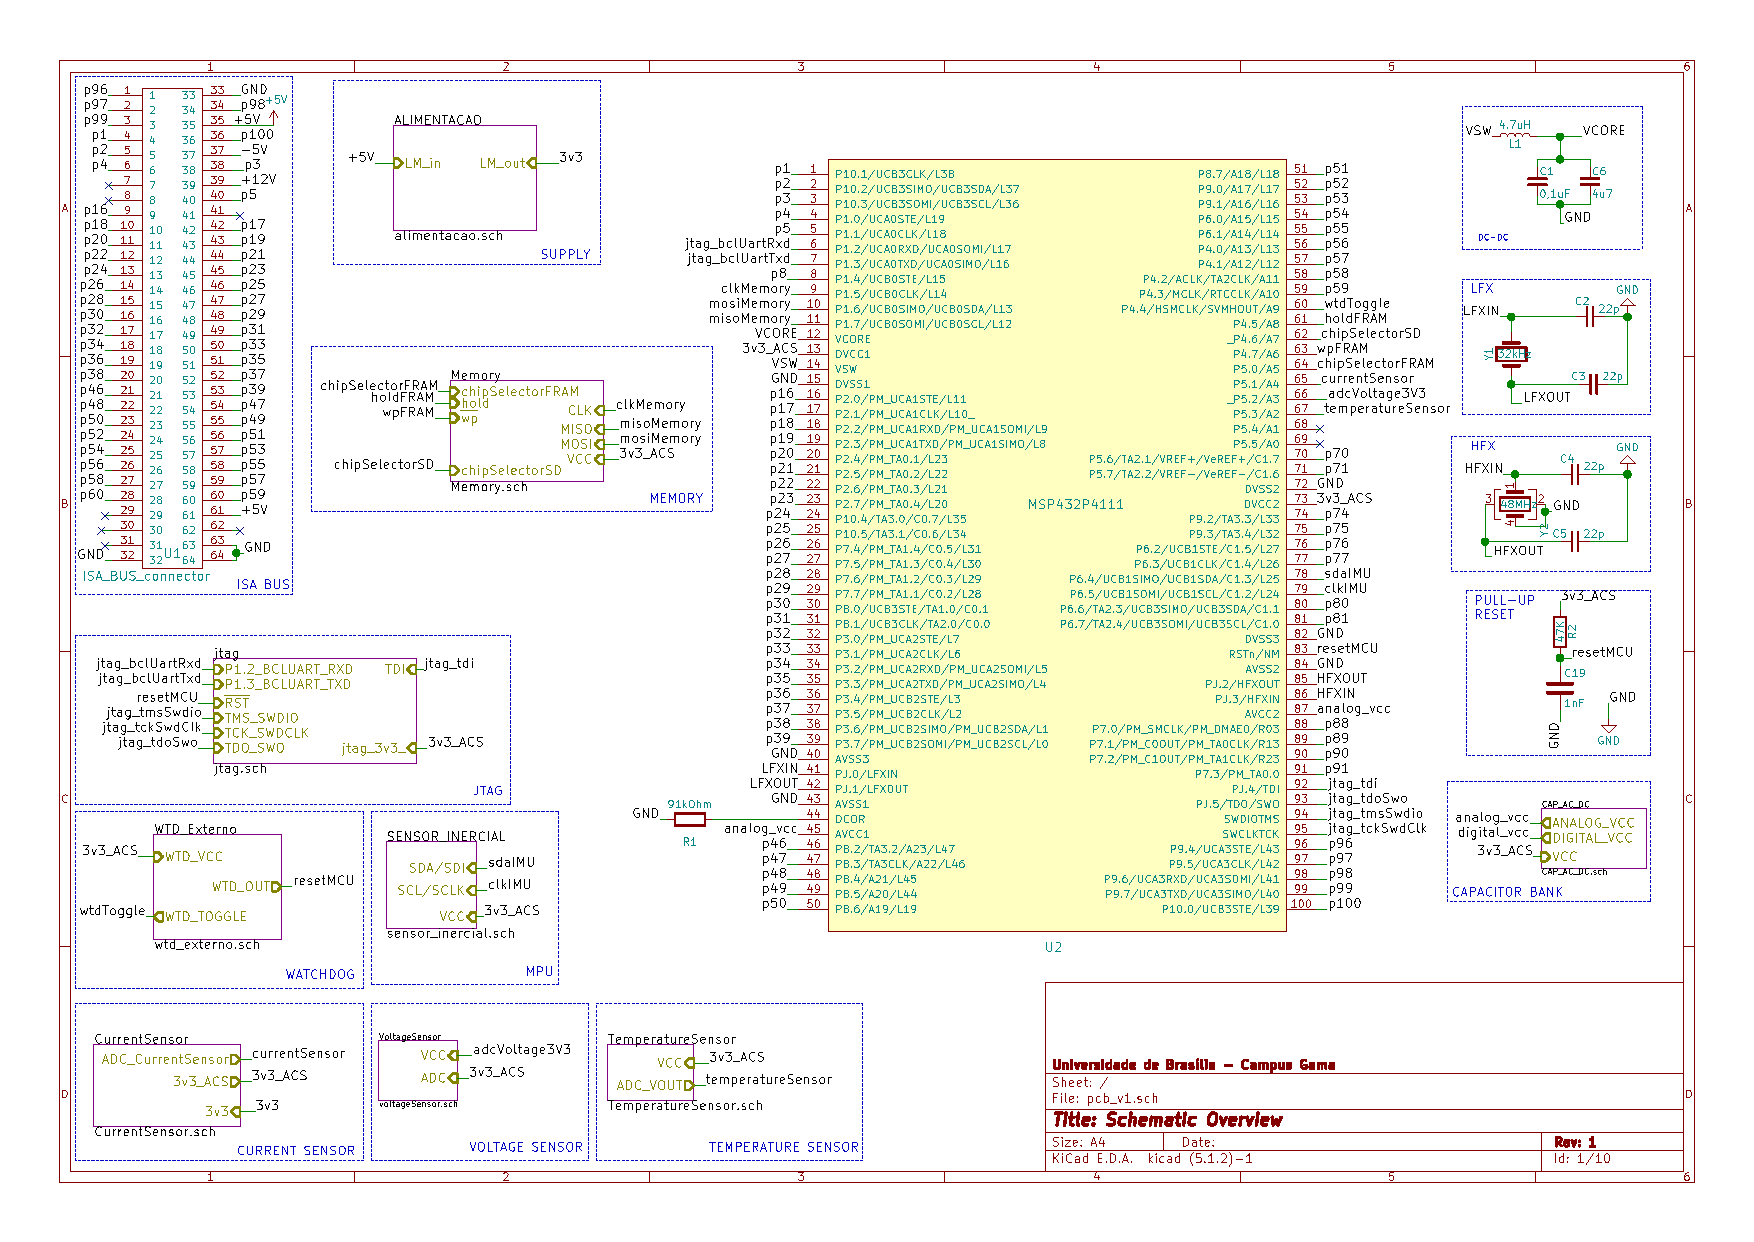
\includepdf[pagecommand={\null\enlargethispage{2\baselineskip}\vfill\captionof{Esquemático Eletrônico do OBC.}}]{pcb_v1.pdf}
%\includepdf[pagecommand={\null\vfill\captionof{table}{blub}}]{example-image}


\begin{figure}[h]
	\centering
		\caption{Esquemático Eletrônico do OBC.}
		
	\begin{tabular}{@{}c@{\hspace{.5cm}}c@{}}
		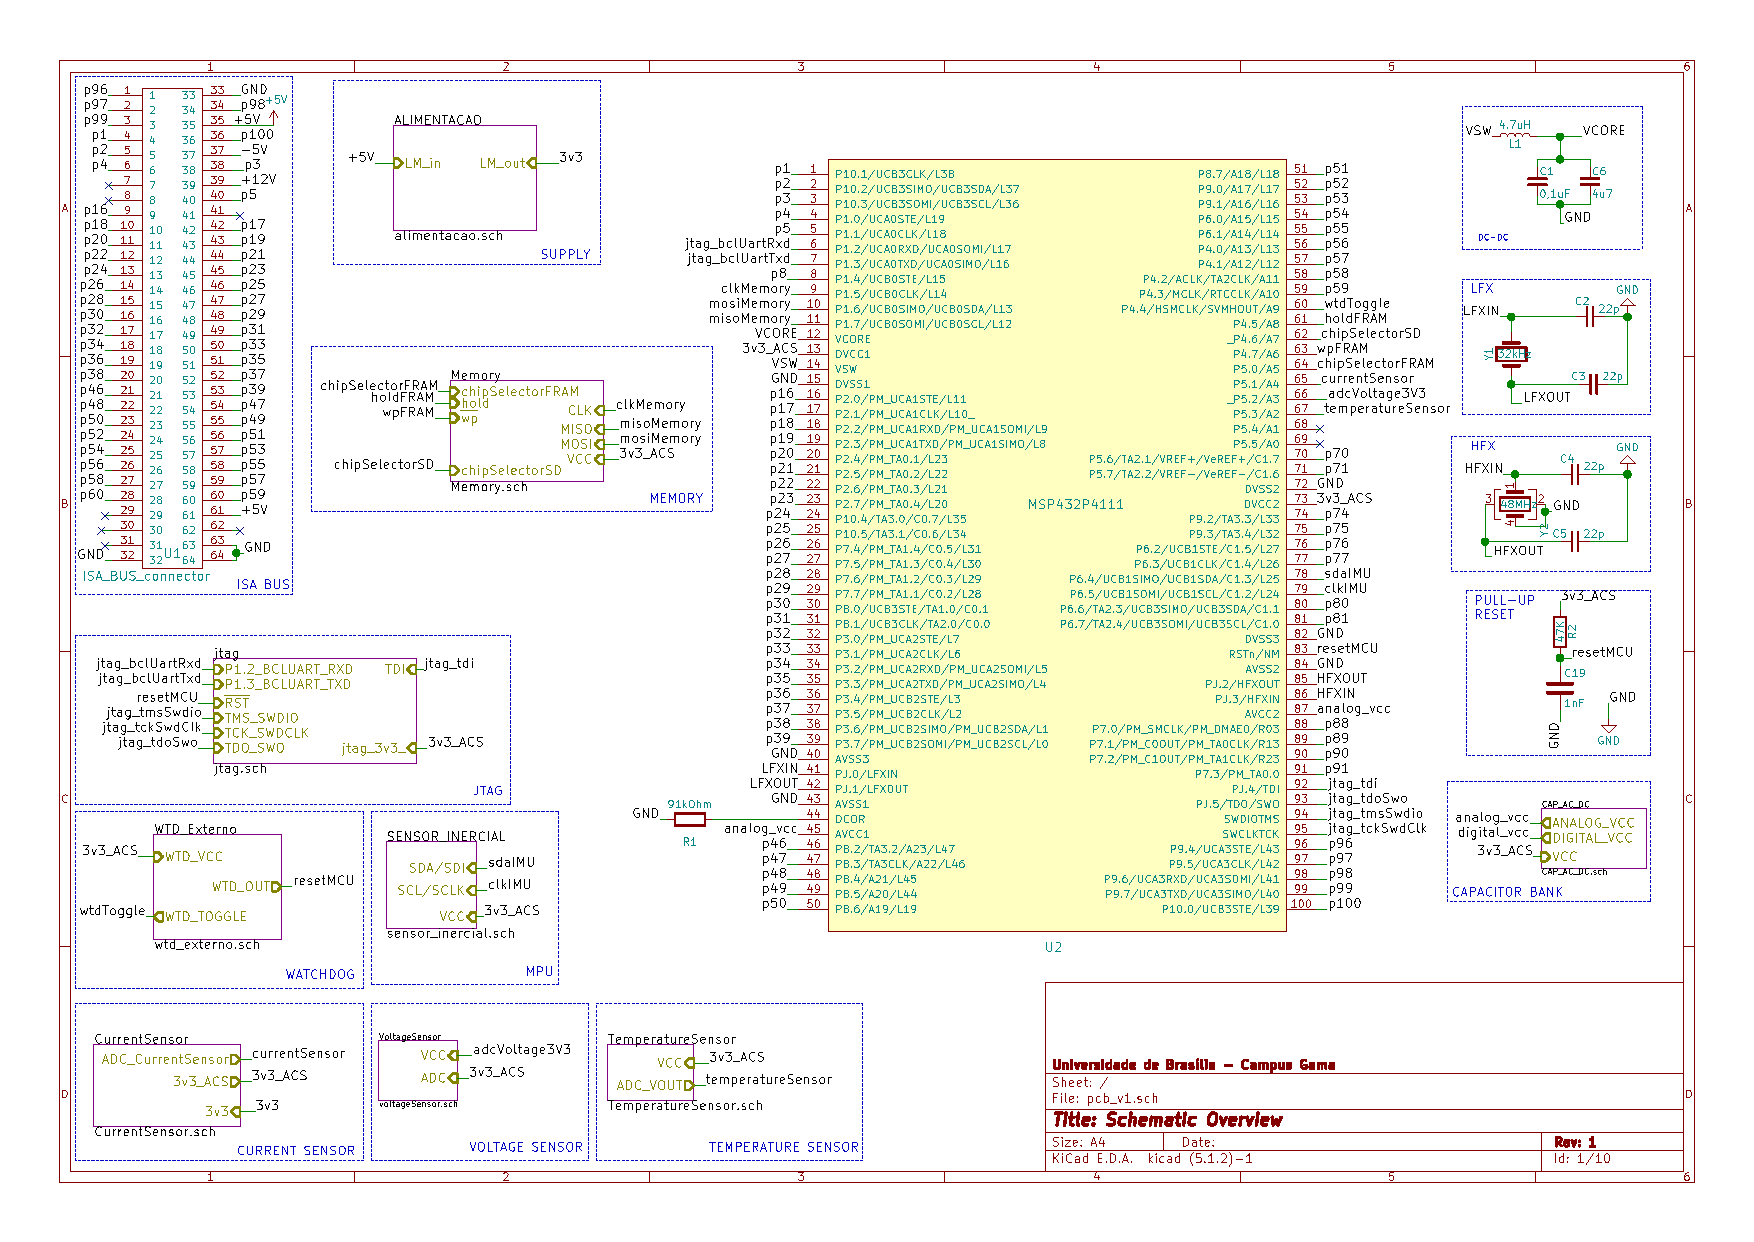
\includegraphics[page=1,width=1.1\textwidth]{pcb_v1.pdf}
	\end{tabular}

	\label{esquematicoObc}
\end{figure}


%\includepdf[pages=1,scale=.9,picturecommand*={\put (\LenToUnit{.05\paperwidth},20) {};}]{}

\newpage

Apos a realização do esquemático, exportou-se o arquivo de conexões (.net) e o importou no ambiente "pcbnew" do KiCad. Esse ambiente permite realizar o roteamento das trilhas, criação de planos de alimentação, etc. Essa foi uma das etapas mais trabalhosas do trabalho pois o roteamento é realizado manualmente. 

Como a soldagem de componentes utilizando maquinas automatizadas é um processo caro e difícil de achar, utilizou-se componentes SMD 1206 (aproximadamente 3.2mm por 1.6mm) para soldar os componentes manualmente. A Figura \ref{pcb_isoView} mostra PCB apos o roteamento e adição das legendas.

\begin{comment}

Para a redução dos custos na soldagem dos componentes, utilizou-se componentes SMD 1206, . Ainda é possibilitável soldar a mão esses componentes.
	content...
\end{comment}

\begin{figure}[h]
	\centering
	\caption{PCB - Vista Isométrica.}
	
	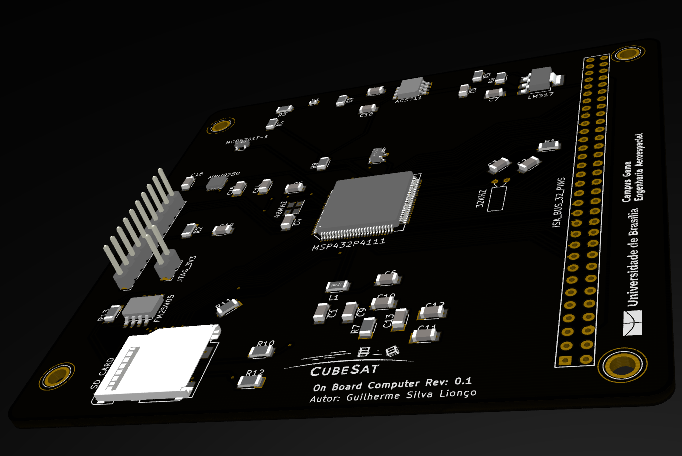
\includegraphics[keepaspectratio=true,scale=0.78]{figuras/pcbRealistic.PNG}
	
	\label{pcb_isoView}
\end{figure}

Alguns componentes não estão presentes na renderização 3D pois não foi possível desenha-los. Não havia tempo suficiente para realizar o desenho. No Apêndice \ref{apendicee} há as imagens do plano de terra e plano de alimentação da PCB.

O BOM (do inglês, \textit{Bill of Material}) também foi exportado da ferramenta e pode ser encontrado no apêndice x. O orçamento dos componentes foi realizado no site Digikey. O valor ficou X, mas o frete ficou y. 


\chapter[DESENVOLVIMENTO DO SOFTWARE]{DESENVOLVIMENTO DO SOFTWARE}

Este capítulo visa descrever o desenvolvimento do \textit{software} embarcado. Inicialmente será mostrado os requisitos e funcionalidades consideradas no desenvolvimento do sistema. Logo em seguida, será exposto a arquitetura utilizada para a aplicação. Após essa etapa, será mostrado com mais detalhes os \textit{softwares} FreeRTOS, DriverLib e a camada de serviço do cliente. 

Tendo em vista que a missão CubeSat ainda está em fase de discussão, a abordagem utilizada no desenvolvimento foi realizar um \textit{software} modular que, a medida que os requisitos se tornem definitivos, as funcionalidades fossem implementadas. Com isso, o \textit{software} desenvolvido servirá para teste do \textit{hardware} e deverá ser atualizado para a missão final.

\section{Requisitos e Funcionalidades}

Para o desenvolvimento de qualquer projeto, a definição dos requisitos é essencial, pois essa etapa influenciará todo o projeto e definirá as expectativas das partes interessadas. Como mencionado acima, poucos requisitos foram delimitados devido à fase inicial da missão CubeSat.

A abordagem utilizada para contornar essa situação foi adicionando requisitos de CubeSats já lançados com alguns requisitos já especificados para a missão, mesma abordagem utilizada na Seção \ref{secaoHardware}.

Com base no Apêndice \ref{apendiceb}, foi possível delimitar as funcionalidades para o \textit{hardware} do sistema. Esses requisitos podem ser vistos na tabela abaixo.

% Please add the following required packages to your document preamble:
% \usepackage{booktabs}
\begin{table}[h]
\centering
\caption{Requisítos do \textit{software} emabarcado.}
\label{tabela_req}
\makebox[1 \textwidth][c]{
\scalebox{0.83}{
\begin{tabular}{@{}cl@{}}
\toprule
\textbf{Número do Requisito} & \multicolumn{1}{c}{\textbf{Descrição do Requisíto}}                                                                                                                                                                                                                                                    \\ \midrule
OBC-SW-R1                    & \begin{tabular}[c]{@{}l@{}}O OBC deve armazenar os seguintes dados a cada um segundo:  Imagens da Carga Útil e\\informações temporais e espaciais das imagens; Temperatura do sistema; Tensão e Corrente\\consumidas pelo sistema; Atitude do CubeSat; Resposta de cada subsistema.\end{tabular} \\\hline
OBC-SW-R2                    & O OBC deve controlar os subsistemas do CubeSat.                                                                                                                                                                                                                                                        \\\hline
OBC-SW-R3                    & O OBC deve realizar um log de eventos do sistema.                                                                                                                                                                                                                                                      \\\hline
OBC-SW-R4                    & \begin{tabular}[c]{@{}l@{}}O OBC deve ter um controle da referência temporal, com uma precisão de 500ms.\end{tabular}                                                                                                                                                                               \\\hline
OBC-SW-R5                    & \begin{tabular}[c]{@{}l@{}}O OBC deve realizar o pacote de telemetria/payload e enviar dados\\  para o subsistema de TT\&C, durante uma janela de transmissão.\end{tabular}                                                                                                                            \\\hline
OBC-SW-R6                    & \begin{tabular}[c]{@{}l@{}}O OBC deve identificar e executar os comandos recebidos da Estação Terrestre.\end{tabular}                                                                                                                                                                               \\\hline
OBC-SW-R7                    & \begin{tabular}[c]{@{}l@{}}O OBC deve alternar os modos de operação de acordo com o a potência na bateria.\end{tabular}                                                                                                                                                                             \\ \hline
OBC-SW-R8                    & O OBC deve possuir um sistema anti travamento.                                                                                                                                                                                                                                                         \\ \bottomrule
\end{tabular}}}
\end{table}


\section{Arquitetura do Software}

A arquitetura de um software é um dos principais pontos a serem definidos em um projeto de \textit{software}, pois a arquitetura influenciará na manutenibilidade e reusabilidade do sistema. Existem várias arquitetura de \textit{software}, sendo as mais usuais: Arquitetura Baseada em Camadas (LBA, do inglês \textit{Layered-based Architecture}), Arquitetura Orientada em Serviços (SOA, do inglês \textit{Service Oriented Architecture}) e a Arquitetura Baseada em Desenvolvimento (CBD, do inglês \textit{Component-based Development}). Dentre essas, a arquitetura que melhor atende os padrões de modularidade é a Arquitetura em Camadas, pois abstrai o \textit{software} embarcado de acordo com sua proximidade com o \textit{hardware} (BACELO, 2010).

	A arquitetura em camadas (do inglês \textit{Layered Architecture}) é muito utilizada em sistemas embarcados, pois ajuda na abstração de alguns componentes e interfaces. Isso faz com que o usuário não precise ter noção de partes muito específicas do sistema, facilitando na usabilidade e na atualização do \textit{software}. A figura abaixo mostra uma arquitetura em camadas de abstração, a mesma que será utilizada no sistema.

\begin{figure}[h]
	\centering
	\caption{Arquitetura de abstração de Camadas.}
	
	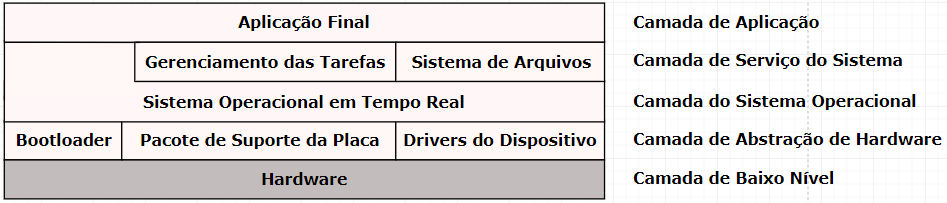
\includegraphics[keepaspectratio=true,scale=0.7]{figuras/arquiteturaSof.PNG}
	
	Fonte: (EBRARY, 2018,  adaptado pág.1).
	\label{fig22}
\end{figure}

Abaixo há uma breve descrição de cada camada e sua aplicação no sistema final.

\begin{itemize}
\item \textbf{Camada de Abstração de Hardware} 

A camada de abstração de \textit{hardware} (HAL, do inglês \textit{Hardware Abstraction Layer}), é uma camada de abstração de \textit{software} entre o \textit{hardware} do sistema embarcado e o sistema operacional. Em geral, o HAL inclui o bootloader, o pacote de suporte de placa, drivers e outros componentes. Ela é a camada de mais baixo nível do \textit{software} embarcado (EBRARY, 2018).

No sistema, a camada de HAL é desempenhada pelo pacote \textit{Driver Library} (\textit{DriverLib}), desenvolvido pela Texas Instruments, que tem o intuito de facilitar o desenvolvimento de projetos embarcados e ajudar na portabilidade dos códigos. Utilizando esse pacote, o desenvolvedor não necessita saber o que acontece a nível de registrador, tornando o desenvolvimento mais amigável e rápido  (TEXAS INSTRUMENTS, 2018).

O \textit{DriverLib} inclui as Interface de Programação de Aplicativos (APIs, do inglês \textit{Application Programming Interface}) das funcionalidades de ADC, Interrupção, UART, entre outros. Esse pacote pode ser também embutido no código final ou não. O MSP432P4111 possui em sua memória ROM uma cópia do \textit{DriverLib}, fazendo com que o pacote não interfira no tamanho do código final.

\item \textbf{Camada do Sistema Operacional}

Um Sistema Operacional de Tempo Real (RTOS, do inglês \textit{Real-Time Operationg System}) é um sistema de \textit{software} que tem a habilidade de prover um serviço em um tempo pré-determinado. O RTOS gerencia uniformemente os recursos da camada inferior, camada HAL, oferecendo esses recursos em forma de serviços (EBRARY,2018).

Escolher um RTOS é uma tarefa importante para dar suporte à interrupções, temporizadores, comunicação entre tarefas, sincronização, gerenciamento de memória, múltiplo acesso, prioridade de execução e escalonamento de tarefas (BASKIYAR ; MEGHANATHAN, 2005).

Analisando o Apêndice \ref{apendicea}, pôde-se afirmar que a maioria das missões utilizavam RTOS, sendo os mais comuns o FreeRTOS e o Linux. Dentre esses, apenas o FreeRTOS possui suporte para o MSP432P4111 pois o Linux necessita de um \textit{hardware} com maior velocidade de clock e maior memória RAM. Tendo esse cenário, o sistema operacional escolhido para o sistema foi o FreeRTOS e ele será explicado mais adiante. 

\item \textbf{Camada de Serviço do Sistema}

A Camada de Serviço do Sistema (CSS) é uma interface que o sistema operacional fornece à Camada de Aplicação Final. Usando essa interface, os aplicativos podem acessar vários serviços fornecidos pelo sistema operacional. Essa camada geralmente inclui o sistema de arquivos, o gerenciador de tarefas, temporizadores, etc (EBRARY,2018).

Nesse caso, o FreeRTOS já oferece APIs para que auxiliam o acesso de suas funcionalidades. Entretanto a CSS não estaria completa só com essas APIS, com isso será há a necessidade de implementar mais funcionalidades nessa camada, levando em consideração os requisitos da Tabela \ref{tabela_req}. Mais adiante, será explicado a proposta de implementação.


\item \textbf{Camada de Aplicação}

A Camada de Aplicação Final (CAF) possui a maior hierarquia da Arquitetura em Camadas. Ela implementa as funcionalidades e tarefas do sistema. De uma forma geral, os níveis abaixo tem o objetivo de auxiliar a CAF (EBRARY, 2018).

Como essa camada realizará tarefas específicas da missão, a necessidade de requisitos da aplicação deverão ser listados. Com isso, a CAF será desenvolvida em versões futuras do \textit{software} embarcado, implementando as funcionalidades exigidas pela missão.



\end{itemize}

\section{DriverLib}

Como mencionado na seção anterior, o \textit{DriverLib} é um conjunto de APIs utilizado para controlar, configurar e manipular os periféricos do microcontrolador, MSP432P411. Além de deixar o código mais intuitivo, esse pacote auxilia a criação de um código de fácil portabilidade entre as plataformas da família MSP432 e MSP430.

Utilizar o \textit{DriverLib} como camada de HAL é vantajoso em virtude de ser uma solução testada por profissionais e bem documentada. O Guia do Usuário do \textit{DriverLib} apresenta um exemplo onde compara a configuração do \textit{MasterClock} à nível de registradores, Código \ref{lst:codigo1}, e utilizando a API-\textit{CS\_initClockSignal()} do \textit{DriverLib}, Código \ref{lst:codigo2}. Com esse exemplo fica evidente o grau de abstração e facilidade que o \textit{DriverLib} oferece.

Como mencionado na seção anterior, o \textit{DriverLib} é um conjunto de APIs utilizado para controlar, configurar e manipular os periféricos do microcontrolador, MSP432P411. Além de deixar o código mais intuitivo, esse pacote auxilia a criação de um código de fácil portabilidade entre as plataformas da família MSP432 e MSP430.


\lstset{
	backgroundcolor=\color{gray!20},%
    basicstyle=\small\ttfamily,%
    numbers=left, numberstyle=\tiny, stepnumber=1, numbersep=2pt,%
    frame=tb, % draw a frame at the top and bottom of the code block
    tabsize=4, % tab space width
    showstringspaces=false, % don't mark spaces in strings
    numbers=left, % display line numbers on the left
    commentstyle=\color{green}, % comment color
    keywordstyle=\color{blue}, % keyword color
    stringstyle=\color{red} % string color
}
\lstset{emph={%  
    CS_initClockSignal
    },emphstyle={\color{blue}\bfseries}%
}%
\renewcommand{\lstlistingname}{Código}
\begin{lstlisting}[caption={Configurando o MasterClock a nível de registrador},label={lst:codigo1},language=C]
int main(void){
//...
CSKEY = 0x695A;
CSCTL |= SELM_1 | DIVM_2;
SKEY = 0;
//...
}
\end{lstlisting}

\begin{lstlisting}[caption={Configurando o MasterClock com a API do DriverLib},label={lst:codigo2},language=C]
int main(void){
//...
CS_initClockSignal(CS_MCLK, CS_VLOCK_SELECT, CS_CLOCL_DIVIDER_32);
//...
}
\end{lstlisting}

A tabela abaixo mostra as vinte e cinco APIs do pacote, assim como  uma breve descrição sobre cada API. Caso o leitor queira se aprofundar na leitura poderá consultar a referência (TEXAS INSTRUMENTSc, 2015). 

\begin{table}[h]
\centering
\caption{Lista de todas as APIs disponíveis no pacote DriverLib.}
\label{my-label}
\makebox[1 \textwidth][c]{
\scalebox{0.61}{
\begin{tabular}{@{}|rl|l|rl|@{}}
\cmidrule(r){1-2} \cmidrule(l){4-5}
\multicolumn{1}{|c}{\textbf{API}} & \multicolumn{1}{c|}{\textbf{Descrição}}                                                                                                                                                                                                                  &  & \multicolumn{1}{c}{\textbf{API}} & \multicolumn{1}{c|}{\textbf{Descrição}}                                                                                                                                                                                           \\ \cmidrule(r){1-2} \cmidrule(l){4-5} 
ADC4                              & \begin{tabular}[c]{@{}l@{}}Permite o controlar os \\ conversores Analógico Digital.\end{tabular}                                                                                                                                                         &  & PMAP                             & \begin{tabular}[c]{@{}l@{}}Essa API permite configurar o modulo Port Mapping \\ Controller. Esse modulo é responsável por \\ reconfigurar as funções digitais de cada porta.\end{tabular}                                         \\
AES256                            & \begin{tabular}[c]{@{}l@{}}Permite a criptografia e descriptografia \\ de dados de 128bits, de acordo com o \\ padrão (AES256)\end{tabular}                                                                                                              &  & PSS                              & \begin{tabular}[c]{@{}l@{}}Permite a configuração das várias entradas de \\ alimentação do microcontrolador, de modo \\ a otimizar a eficiência energética.\end{tabular}                                                          \\
COMP\_E                           & \begin{tabular}[c]{@{}l@{}}Essa API fornece um conjunto de funções \\ para inicializar os módulos COMP\_E,\\ de comparação de dois sinais de entrada analógicos.\end{tabular}                                                                            &  & REF\_A                           & \begin{tabular}[c]{@{}l@{}}Permite configurar e ativar o uso da tensão de \\ referência REF\_A\end{tabular}                                                                                                                       \\
CRC32                             & \begin{tabular}[c]{@{}l@{}}Permite fornecer um conjunto de funções para \\ a verificação de dados. Essas funções são uteis \\ quando há a necessidade de verificar a acurácia \\ de um dado recebido em um canal de comunicação.\end{tabular}            &  & ResetCtl                         & \begin{tabular}[c]{@{}l@{}}Permite configurar e manipular as funções do reset \\ do microcontrolador, tanto soft reset quanto \\ hard reset.\end{tabular}                                                                         \\
CS                                & \begin{tabular}[c]{@{}l@{}}Permite controlar o sistema de clock do \\ microcontrolador.\end{tabular}                                                                                                                                                     &  & RTC\_C                           & \begin{tabular}[c]{@{}l@{}}Essa API fornece um conjunto de funções para \\ controlar o Real Time Clock (RTC\_C).\end{tabular}                                                                                                     \\
DMA                               & \begin{tabular}[c]{@{}l@{}}Essa API permite controlar o Direct \\ Memory Access (DMA) do microcontrolador, \\ permitindo transferir blocos de dados \\ sem a necessidade de utilizar o processamento\\  do microcontrolador.\end{tabular}                &  & SPI                              & \begin{tabular}[c]{@{}l@{}}Essa API fornece o controle do barramento \\ eUSCI\_A/eUSCI\_B, no modo SPI, permitindo a \\ configuração da frequência de transmissão, \\ envio/recebimento de dados, status, etc.\end{tabular}       \\
FlashCtl                          & \begin{tabular}[c]{@{}l@{}}Permite o controlar o processo de gravar, \\ apagar e configurar a memória interna do processador.\end{tabular}                                                                                                               &  & SysCtl                           & \begin{tabular}[c]{@{}l@{}}Essa API junta os módulos do sistema que não \\ se encaixam em nenhum periférico especifico.\end{tabular}                                                                                              \\
FPU                               & \begin{tabular}[c]{@{}l@{}}Essa API fornece métodos para manipular o \\ comportamento da Unidade de Ponto Flutuante \\ (FPU do inglês Floating-Point Unit) do \\ processador Cortex-M.\end{tabular}                                                      &  & SysTick                          & \begin{tabular}[c]{@{}l@{}}O SysTick é um temporizador simples que fornece\\ uma interrupção periódica para RTOS, mas ele \\ pode ser usado para outros fins de temporização.\end{tabular}                                        \\
GPIO                              & \begin{tabular}[c]{@{}l@{}}Permite configurar e ativar os pinos de entrada/saída \\ do microcontrolador e configurar as interrupções.\end{tabular}                                                                                                       &  & Timer32                          & \begin{tabular}[c]{@{}l@{}}Permite a configuração do \\ Timer32 (contador de 32 bits).\end{tabular}                                                                                                                               \\
I2C                               & \begin{tabular}[c]{@{}l@{}}Essa API fornece o controle do barramento eUSCI\_B, \\ no modo I2C, permitindo a configuração da frequência \\ de transmissão, envio/recebimento de dados, status, etc.\end{tabular}                                          &  & Timer\_A                         & \begin{tabular}[c]{@{}l@{}}Essa API permite configurar o modulo TimerA. \\ Esse modulo é um temporizador/contador de 16 bits, \\ suportando múltiplos modos captura/comparação, \\ PWM e temporização de intervalos.\end{tabular} \\
NVIC                              & \begin{tabular}[c]{@{}l@{}}Permite controlar o Nested Vectored Interrupt \\ Controller (NVIC). Esse modulo ativa, desativa, registra e \\ configura as prioridades das interrupções do microcontrolador.\end{tabular}                                    &  & UART                             & \begin{tabular}[c]{@{}l@{}}Essa API fornece o controle do barramento \\ serial USCI, permitindo a configuração \\ da frequência de transmissão, envio/recebimento \\ de dados, status, etc.\end{tabular}                          \\
MPU                               & \begin{tabular}[c]{@{}l@{}}Essa API fornece funções para configurar o \\ Memory Protection Unit (MPU). O MPU é acoplado \\ ao núcleo do processador Cortex-M e fornece um meio de \\ estabelecer permissões de acesso à regiões da memória.\end{tabular} &  & WDT\_A                           & Permite o controle do Watchdog padrão do sistema.                                                                                                                                                                                 \\
PCM                               & \begin{tabular}[c]{@{}l@{}}Permite o gerenciamento dos estados de \\ energia do microcontrolador.\end{tabular}                                                                                                                                           &  & \multicolumn{1}{l}{}             &                                                                                                                                                                                                                                   \\ \cmidrule(r){1-2} \cmidrule(l){4-5} 
\end{tabular}}}
\end{table}

\newpage

\section{FreeRTOS}

O \textit{FreeRTOS} é um kernel (gerenciador) utilizado em aplicações embarcadas que necessitam de aplicação em tempo real, sendo normalmente empregado em CubeSats. Esse kernel, desenvolvido e mantido pela Real Time Engineers Ltd, é distribuído gratuitamente sobre a licença \textit{General Public License} (GPL) (BARRY, 2016). O \textit{FreeRTOS} foi desenvolvido para ser pequeno, portátil e escalável; de acordo com o site oficial\footnote{Disponível em \url{https://www.freertos.org}. Acesso em: 18/06/2018} o kernel possui uma imagem típica de 6K a 12K bytes.

O FreeRTOS é utilizado tanto em sistemas Não Críticos de Tempo Real (Soft-RTOS), quanto em sistemas Críticos de Tempo Real (Hard-RTOS). Aplicações Soft-RTOS possuem um tempo específico para a realização de uma tarefa, mas o não cumprimento do prazo de execução não causa uma falha no sistema. Por exemplo, caso as luzes internas do carro não acenderem no instante em que a porta for aberta, o usuário não estaria em risco. Já as aplicações Hard-RTOS, o não cumprimento do prazo resulta em falha do sistema. Por exemplo, se o sensor de colisão do carro atrasar a sua resposta, o usuário estaria em grande risco (BARRY, 2016).

No caso de aplicações aeroespaciais, o sistema deve ser projetado para ser um Hard-RTOS pois o travamento do \textit{software} embarcado ocasionaria em falha total do sistema. Foi percebido que todas as missões pesquisadas, Apêndice \ref{apendiceb}, possuíam algum tipo de sistema operacional para gerenciar as tarefas embarcadas.

No FreeRTOS, cada tarefa em execução é chamada de ‘\textit{task}’. Para manter um padrão, será utilizada essa nomenclatura. No contexto do projeto, o uso das tasks é fundamental para criar um certo nível de abstração e garantir o requisito de Hard-RTOS. Por exemplo, a leitura da tensão da bateria é de extrema importância, então ela possuirá maior prioridade em relação a task de envio de dados; pois se o satélite consumir por completo a carga da bateria, ocasionando na perda do satélite .

Uma task só pode estar em quatro estados: \textit{Ready}, \textit{Running}, \textit{Suspend} e \textit{Blocked}. As APIs são encarregadas de alterar os estados de cada \textit{task}. Os estados são melhores ilustrados na figura abaixo, onde há evidenciado as APIs responsáveis pela mudança.

\begin{figure}[h]
	\centering
	\caption{Estados das Tasks no FreeRTOS}
	 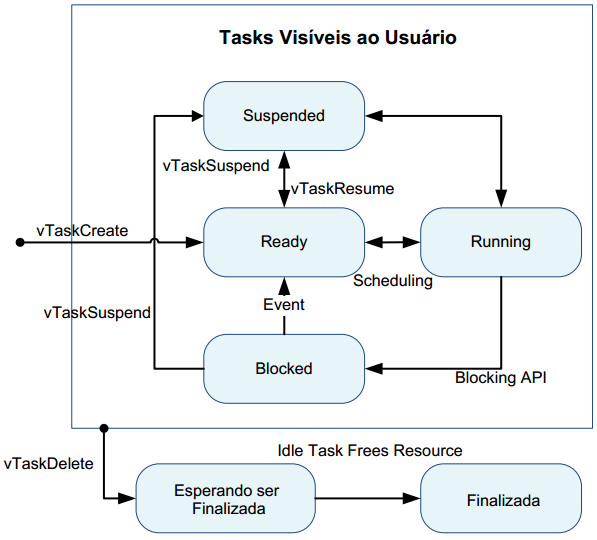
\includegraphics[keepaspectratio=true,scale=0.8]{figuras/freertosTasks.PNG}
	 
	 Fonte: (LIN,2010, adaptado pág.20)
	
	\label{fig23}
\end{figure}

\subsection{APIs do FreeRTOS}

As APIs do FreeRTOS foram criadas para facilitar o desenvolvimento, fazendo uma interface entre o usuário e o kernel. De acordo com o site oficial há 145 APIs que são agrupadas nas seguintes categorias:

\begin{itemize}
\item\textit{Task Creation}, permite que o usuário crie ou elimine uma \textit{task} do sistema.
\item\textit{Task Control}, permite a troca dos estados das \textit{task}.
\item\textit{Task Utilities}, possui APIs que APIs que permitem o usuário pegar alguma informação sobre as \textit{task}, por exemplo, quais \textit{task} estão em execução.
\item\textit{RTOS Kernel Control}, essa API oferece controle sobre o \textit{kernel}, permitindo o usuário começar o \textit{task scheduler},  suspender as \textit{task} em execução, entre outros.
\item\textit{Direct To Task Notifications} , permite a troca de mensagens entre as \textit{task}.
\item\textit{FreeRTOS-MPU Specific}, possui 3 APIs que permitem o usuário realizar o controle do \textit{kernel} MPU.
\item\textit{Queues}, permite a comunicação entre as tarefas e interrupções a partir de uma fila.
\item\textit{Queue Sets}, permite o controle mais geral das filas, por exemplo, bloqueio de acesso das tarefas às filas.
\item\textit{Semaphore/Mutexes}, permite que usuário use semáforos binários para sincronização.
\item\textit{Software Timers,} permite a utilização de temporizadores, muito utilizado para contabilizar o tempo gasto entre as \textit{task}.
\item\textit{Event Group}, essas APIs são flags que indicam se um evento ocorreu ou não, sendo muito utilizado para a gerar logs do sistema.
\item\textit{Co-routines}, permite a criação de rotinas, uma alternativa para tarefas com pouca prioridade.
\end{itemize}

Descrever cada API do \textit{kernel} seria um tarefa cansativa e desnecessária, uma vez que há o manual de referência que explica cada uma e ainda mostra alguns exemplos. Com isso, abaixo há uma tabela que contém a descrição das funcionalidades das APIs das categorias \textit{Task Creation} e \textit{Task Control}. Essas categorias foram escolhidas para serem tratadas no texto, pois a manipulação das tarefas é a ação mais usual em um projeto com o FreeRTOS.

Abaixo há uma breve descrição sobre as APIs das categorias \textit{Task Creation} e \textit{Task Control}.

\begin{table}[h]
\centering
\caption{APIs da categoria Task Control e Task Creation.}
\label{my-label}
\makebox[1 \textwidth][c]{
\scalebox{0.66}{
\begin{tabular}{@{}cll@{}}
\toprule
\textbf{Categoria}             & \multicolumn{1}{c}{\textbf{Nome da API}} & \textbf{Funcionalidade}                                                                                                                                                                                                             \\ \midrule
\multirow{3}{*}{Task Creation} & xTaskCreate()                            & \begin{tabular}[c]{@{}l@{}}Criação de uma task com sua prioridade. \\ Se a prioridade for maior que a task em \\ execução, a task criada começa sua \\ execução. A API retorna um handler\\ para a tarefa.\end{tabular}             \\ \cmidrule(l){2-3} 
                               & xTaskCreateStatic()                      & \begin{tabular}[c]{@{}l@{}}Cria uma task, semelhante ao xTaskCreate. \\ Entretanto, o tamanho destinado para a \\ RAM é definido pelo usuário e é alocado \\ estaticamente. A API retorna um handler \\ para a tarefa.\end{tabular} \\ \cmidrule(l){2-3} 
                               & vTaskDelete()                            & \begin{tabular}[c]{@{}l@{}}Realiza a remoção da tarefa. Se a task \\ estiver em execução, o kernel  busca \\ uma tarefa de maior prioridade para \\ ser executada.\end{tabular}                                                     \\ \midrule
\multirow{8}{*}{Task Control}  & vTaskDelay()                             & \begin{tabular}[c]{@{}l@{}}Coloca a task, que está em execução, \\ no modo Blocked e aciona o timer para \\ despertar.\end{tabular}                                                                                                 \\ \cmidrule(l){2-3} 
                               & vTaskDelayUntil()                        & \begin{tabular}[c]{@{}l@{}}Coloca uma tarefa em execução no \\ estado de Blocked e configura o \\ tempo de resumo.\end{tabular}                                                                                                     \\ \cmidrule(l){2-3} 
                               & uxTaskPriorityGet()                      & \begin{tabular}[c]{@{}l@{}}Retorna a prioridade da task a partir \\ do seu handler.\end{tabular}                                                                                                                                    \\ \cmidrule(l){2-3} 
                               & vTaskPrioritySet()                       & \begin{tabular}[c]{@{}l@{}}Define uma nova prioridade para \\ a task.\end{tabular}                                                                                                                                                  \\ \cmidrule(l){2-3} 
                               & vTaskSuspend()                           & \begin{tabular}[c]{@{}l@{}}Coloca a task em modo Supended e \\ localiza outra tarefa com prioridade \\ maior para ser executada.\end{tabular}                                                                                       \\ \cmidrule(l){2-3} 
                               & vTaskResume()                            & \begin{tabular}[c]{@{}l@{}}Coloca a tarefa suspensa para o estado \\ de Ready.\end{tabular}                                                                                                                                         \\ \cmidrule(l){2-3} 
                               & xTaskResumeFromISR()                     & \begin{tabular}[c]{@{}l@{}}Coloca a tarefa suspensa no estado de \\ Ready quando o Scheduler estiver \\ parado.\end{tabular}                                                                                                        \\ \cmidrule(l){2-3} 
                               & xTaskAbortDelay()                        & \begin{tabular}[c]{@{}l@{}}Força uma tarefa a sair do modo \\ Blocked e entrar no Ready\end{tabular}                                                                                                                                \\ \bottomrule
\end{tabular}}}
\end{table}

\newpage

\subsection{Configuração do FreeRTOS}

Como o kernel do FreeRTOS é comum para a maioria dos microcontroladores, o porting é essencial para adaptar o kernel para o tipo de microcontrolador usado. No site da empresa há um template do arquivo portmacro.h para o MSP432. Foram modificados poucos parametros, pois o aluno estava se adaptando à tecnologia.


\section{Desenvolvimento da Camada de Serviços do Sistema}

A Linguagem de Modelagem Unificada (UML, do inglês \textit{Unified Modeling Language}) foi escolhida para a estruturação da CSS. Essa ferramenta permite representar graficamente as características de um sistema, como: requisitos, especificações, estruturas, comportamentos, entre outros (BOOSH, 2005). Escolheu-se essa linguagem devido os seguintes fatores:

\begin{itemize}
\item rápido entendimento do \textit{software} a partir do diagrama UML;

\item fácil manutenção do \textit{software};

\item portabilidade do \textit{software} para várias plataformas e linguagens;

\item linguagem de modelagem amplamente utilizada na engenharia de \textit{software}.
\end{itemize}

 
Com as características acima, fica evidente que a UML ajuda na padronização, rápida compreensão e escalabilidade do sistema. Tais pontos são primordiais para versões futuras do \textit{software} embarcado, pois os desenvolvedores não perderam tanto tempo para entender o sistema ou até mesmo tendo que reescrever o sistema novamente. Entretanto, alguns pontos devem ser levados em consideração antes de usar a UML para modelar \textit{software} embarcado.

	O uso da UML ocorre majoritariamente em \textit{softwares} que possuem programação Orientada a Objetos (OO), pois essa modelagem foi baseada no paradigma de orientação a objetos. No contexto do projeto, o intuito é utilizar programação estrutura. Algumas extensões da UML, também chamados de perfis da UML, permitem implementar funcionalidades adicionais para um propósito específico.
    
De acordo com Douglass (2009), o \textit{FunctionalC} é a extensão da UML que permite a modelagem de sistemas baseados na linguagem C. Os diagramas primários desta extensão são mostrados na Tabela \ref{functionalC}. 


\begin{table}[h]
\centering

\caption{Perfil do Diagrama FunctionalC.}
\label{functionalC}
\makebox[1 \textwidth][c]{
\scalebox{0.8}{
\begin{tabular}{cccl}
\hline
\textbf{Tipo de Diagrama}      & \textbf{Diagrama FuncionalC} & \textbf{Diagrama UML}   & \multicolumn{1}{c}{\textbf{Descriçao}}                                                                                                                                                                          \\ \hline
Requisitos                     & Diagrama de Caso de Uso      & Diagrama de Caso de Uso & \begin{tabular}[c]{@{}l@{}}Representa os usos do sistema com relação \\ aos atores.\end{tabular}                                                                                                                 \\ \hline
\multirow{4}{*}{Estrutura}     & Diagrama de Construção       & Diagrama de Componente  & \begin{tabular}[c]{@{}l@{}}Mostra o conjunto de artefatos construídos\\ a partir dos arquivos de origem, como \\ executáveis e bibliotecas.\end{tabular}                                                         \\
                               & Gráfico de Chamadas          & Diagrama de Classes     & \begin{tabular}[c]{@{}l@{}}Mostra as chamadas e suas sequências \\ entre conjuntos de funções.\end{tabular}                                                                                                      \\
                               & Diagrama de Arquivos         & Diagrama de Classes     & \begin{tabular}[c]{@{}l@{}}Mostra o conjunto de arquivos .c e .h \\ e suas relações.\end{tabular}                                                                                                                \\
                               & Diagrama do Código           & nenhum                  & Mostra o código-fonte gerado.                                                                                                                                                                                    \\ \hline
\multirow{3}{*}{Comportamento} & Diagrama de Mensagens        & Diagrama Sequencial     & \begin{tabular}[c]{@{}l@{}}Mostra sequências de chamadas e \\ eventos enviados entre um conjunto \\ de arquivos, incluindo valores de \\ parâmetros passados.\end{tabular}                                       \\
                               & Maquina de Estados           & Diagrama de Estados     & \begin{tabular}[c]{@{}l@{}}Mostra a máquina de estado para \\ arquivos e como suas funções \\ e ações incluídas são executadas \\ à medida que eventos (síncronos ou \\ assíncronos) são recebidos.\end{tabular} \\
                               & Fluxograma                   & Diagrama de Atividades  & \begin{tabular}[c]{@{}l@{}}Detalha o fluxo de controle para\\  uma função ou caso de uso.\end{tabular}                                                                                                           \\ \hline
\end{tabular}}}
Fonte: (DOUGLASS, pag 3,2009).
\end{table}

Para ilustrar como é realizada a implementação de um diagrama UML em linguagem C, o considera-se um arquivo Timer, que tem o objetivo de atualizar o tempo. Ele possui como atributo os segundos e minutos, bem como métodos e operações, como: Reset() e Tick().  A função Reset() poderia inicializar as variáveis para zero, e a função Tick() poderia incrementar o tempo a cada segundo. Em UML esse elemento seria representado conforme a Figura \textcolor{blue}{25}. Em C++ seria realizado uma classe, mas em C seria implementado conforme mostra o Código \ref{lst:codigo3}.

\begin{figure}[h]
\centering
\caption{Exemplo Timer UML.}
	
\begin{tikzpicture}
\label{UML_timer}
\centering
\begin{class}[text width =5cm ]{<Timer>}{0 ,0}
\centering
\attribute {+ mins : int}
\attribute {+ secs : int}
\operation {- tick(): void}
\operation {- reset(): void}
\end{class}
\end{tikzpicture}

Fonte: (DOUGLASS, 2009, pág.5).\linebreak

\end{figure}


\renewcommand{\lstlistingname}{Código}


\begin{lstlisting}[caption={Transcrição do Timer UML para código em C.},label={lst:codigo3},language=C]
extern int mins; 
extern int secs;

/*## operation Reset() */
void reset();

/*## operation tick() */
void tick();

\end{lstlisting}
\begin{center}
Fonte: (DOUGLASS, 2009, pág.5).
\end{center}

\subsection{Desenvolvimento da UML}

Analisando os requisitos do sistema, Tabela \ref{tabela_req}, foi possível abstrair as funções principais exigidas para o software: Controle das Tarefas, Coleta de Dados e Armazenamento. Sendo assim, foram realizado a Maquina de Estados, Fluxograma e o Diagrama de Arquivos necessário para o software embarcado. 

\begin{itemize}

\item \textbf{Maquina de Estados}

A maquina de estados desenvolvida levou em consideração os casos macros do CubeSat em sua orbita. Não foi levado em consideração os estágios de pre-lançamento e \textit{deployment}. Foram considerados quatro modos de operação: \textbf{Nominal Mode}, \textbf{Safe Mode}, \textbf{Battery Low Level Mode} e \textbf{Hibernate Mode}. Esses modos são mostrados na Figura \ref{uml_me}

\begin{figure}[h]
	\centering
	\caption{Maquina de Estados da Camada de Serviço.}
	
	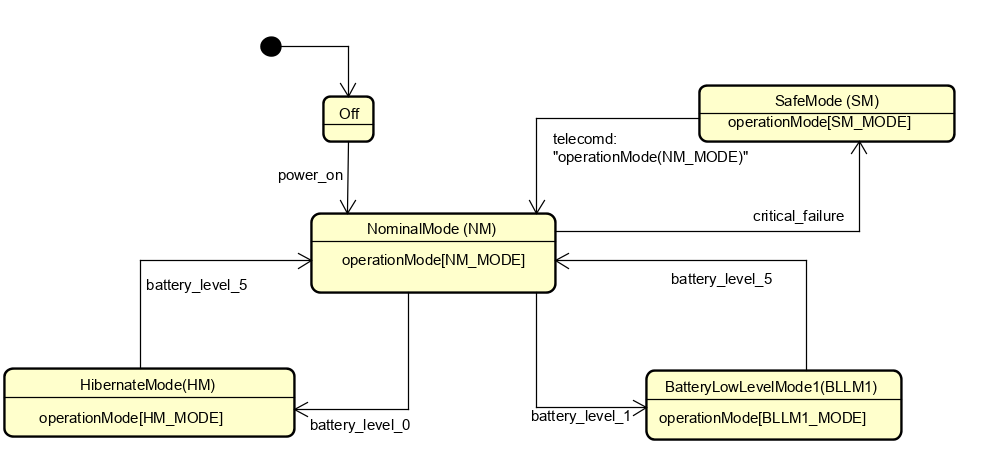
\includegraphics[keepaspectratio=true,scale=0.62]{figuras/stateMachine.png}
	
	\label{uml_me}
\end{figure}

\item \textbf{Fluxograma}

Como o \textit{kernel} escolhido foi o \textit{FreeRTOS} as atividades do OBC foi divididas em \textit{Tasks}. A CCS possui 8 rotinas, sendo: uma de controle (\textbf{TaskManager}); uma de coleta de dados (\textbf{HouseKeeping}); uma de armazenamento (\textbf{DataStorage}); uma de controle de travamento (\textbf{WatchDogTask}); cinco de referentes à camada de aplicação. A Figura \ref{uml_floxograma} mostra o fluxograma de inicialização do sistema e no Apencice \ref{apendicef} há os demais fluxogramas da CSS. 

\begin{figure}[h]
	\centering
	\caption{Fluxograma de Inicialização do sistema.}
	
	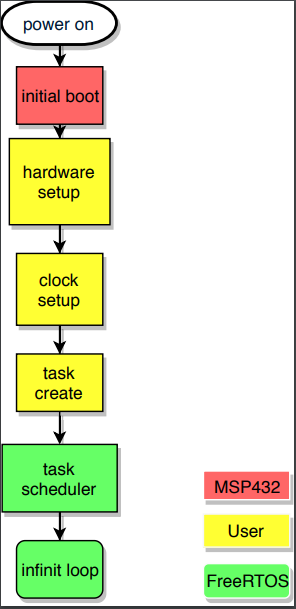
\includegraphics[keepaspectratio=true,scale=0.6]{figuras/flowChart_obc.png}
	
	\label{uml_floxograma}
\end{figure}


\newpage

\item \textbf{Diagrama de Arquivos}

O diagrama de arquivos é semelhante ao diagrama de classes em orientação à objetos. Devido a complexidade do sistema, alguns arquivos ainda estão sendo finalizados. A figura \ref{uml_da} mostra o Diagrama de Arquivos.

\begin{figure}[h]
	\centering
	\caption{Diagrama de Arquivos do Sistema.}
	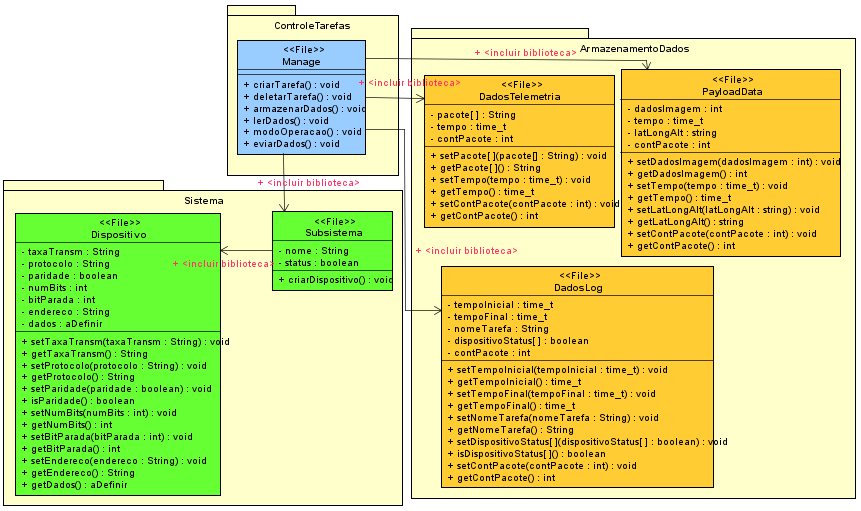
\includegraphics[keepaspectratio=true,scale=0.3]{figuras/CSS.png}
	
	\label{uml_da}
\end{figure}

\begin{comment}
\item \textbf{Desenvolvimento do Fluxograma}

O desenvolvimento do Fluxograma será realizado no TCC2.
\end{comment}


\end{itemize}


\section{Desenvolvimento do Código}

Com base na UML e no diagrama de interface do hardware foi realizado o código embarcado. Vale a pena ressaltar que como a metodologia de desenvolvimento utilizada foi co-design, o desenvolvimento do código foi realizado em paralelo com o desenvolvimento do hardware. 

O Ambiente de Desenvolvimento (IDE, do ingles \textit{Integrated Development Environment}) escolhido foi o \textit{Code Composer Studio}, devido seu amplo uso ... Todo o código foi colocado no repositório\footnote{Código disponível em: \url{https://github.com/guilionzzo/firmware_onBoardComputer/tree/master}} do aluno no GitHub. 

\chapter[RESULTADOS E DISCUSSÃO]{RESULTADOS E DISCUSSÃO}

Até o presente momento, as duas instituições estão discutindo os acordos da parceria. Esse fato impossibilitou a capitação de recursos para a compra dos componentes eletrônicos e fabricação da PCB. Sendo assim, os resultados apresentados serão pertinentes ao teste em protoboard, utilizando a LaunchPad do MSP432 e alguns módulos COTS.

A Figura abaixo mostra a conexão dos componentes na LaunchPad.

\begin{figure}[h]
	\centering
	\caption{Protoboard.}
	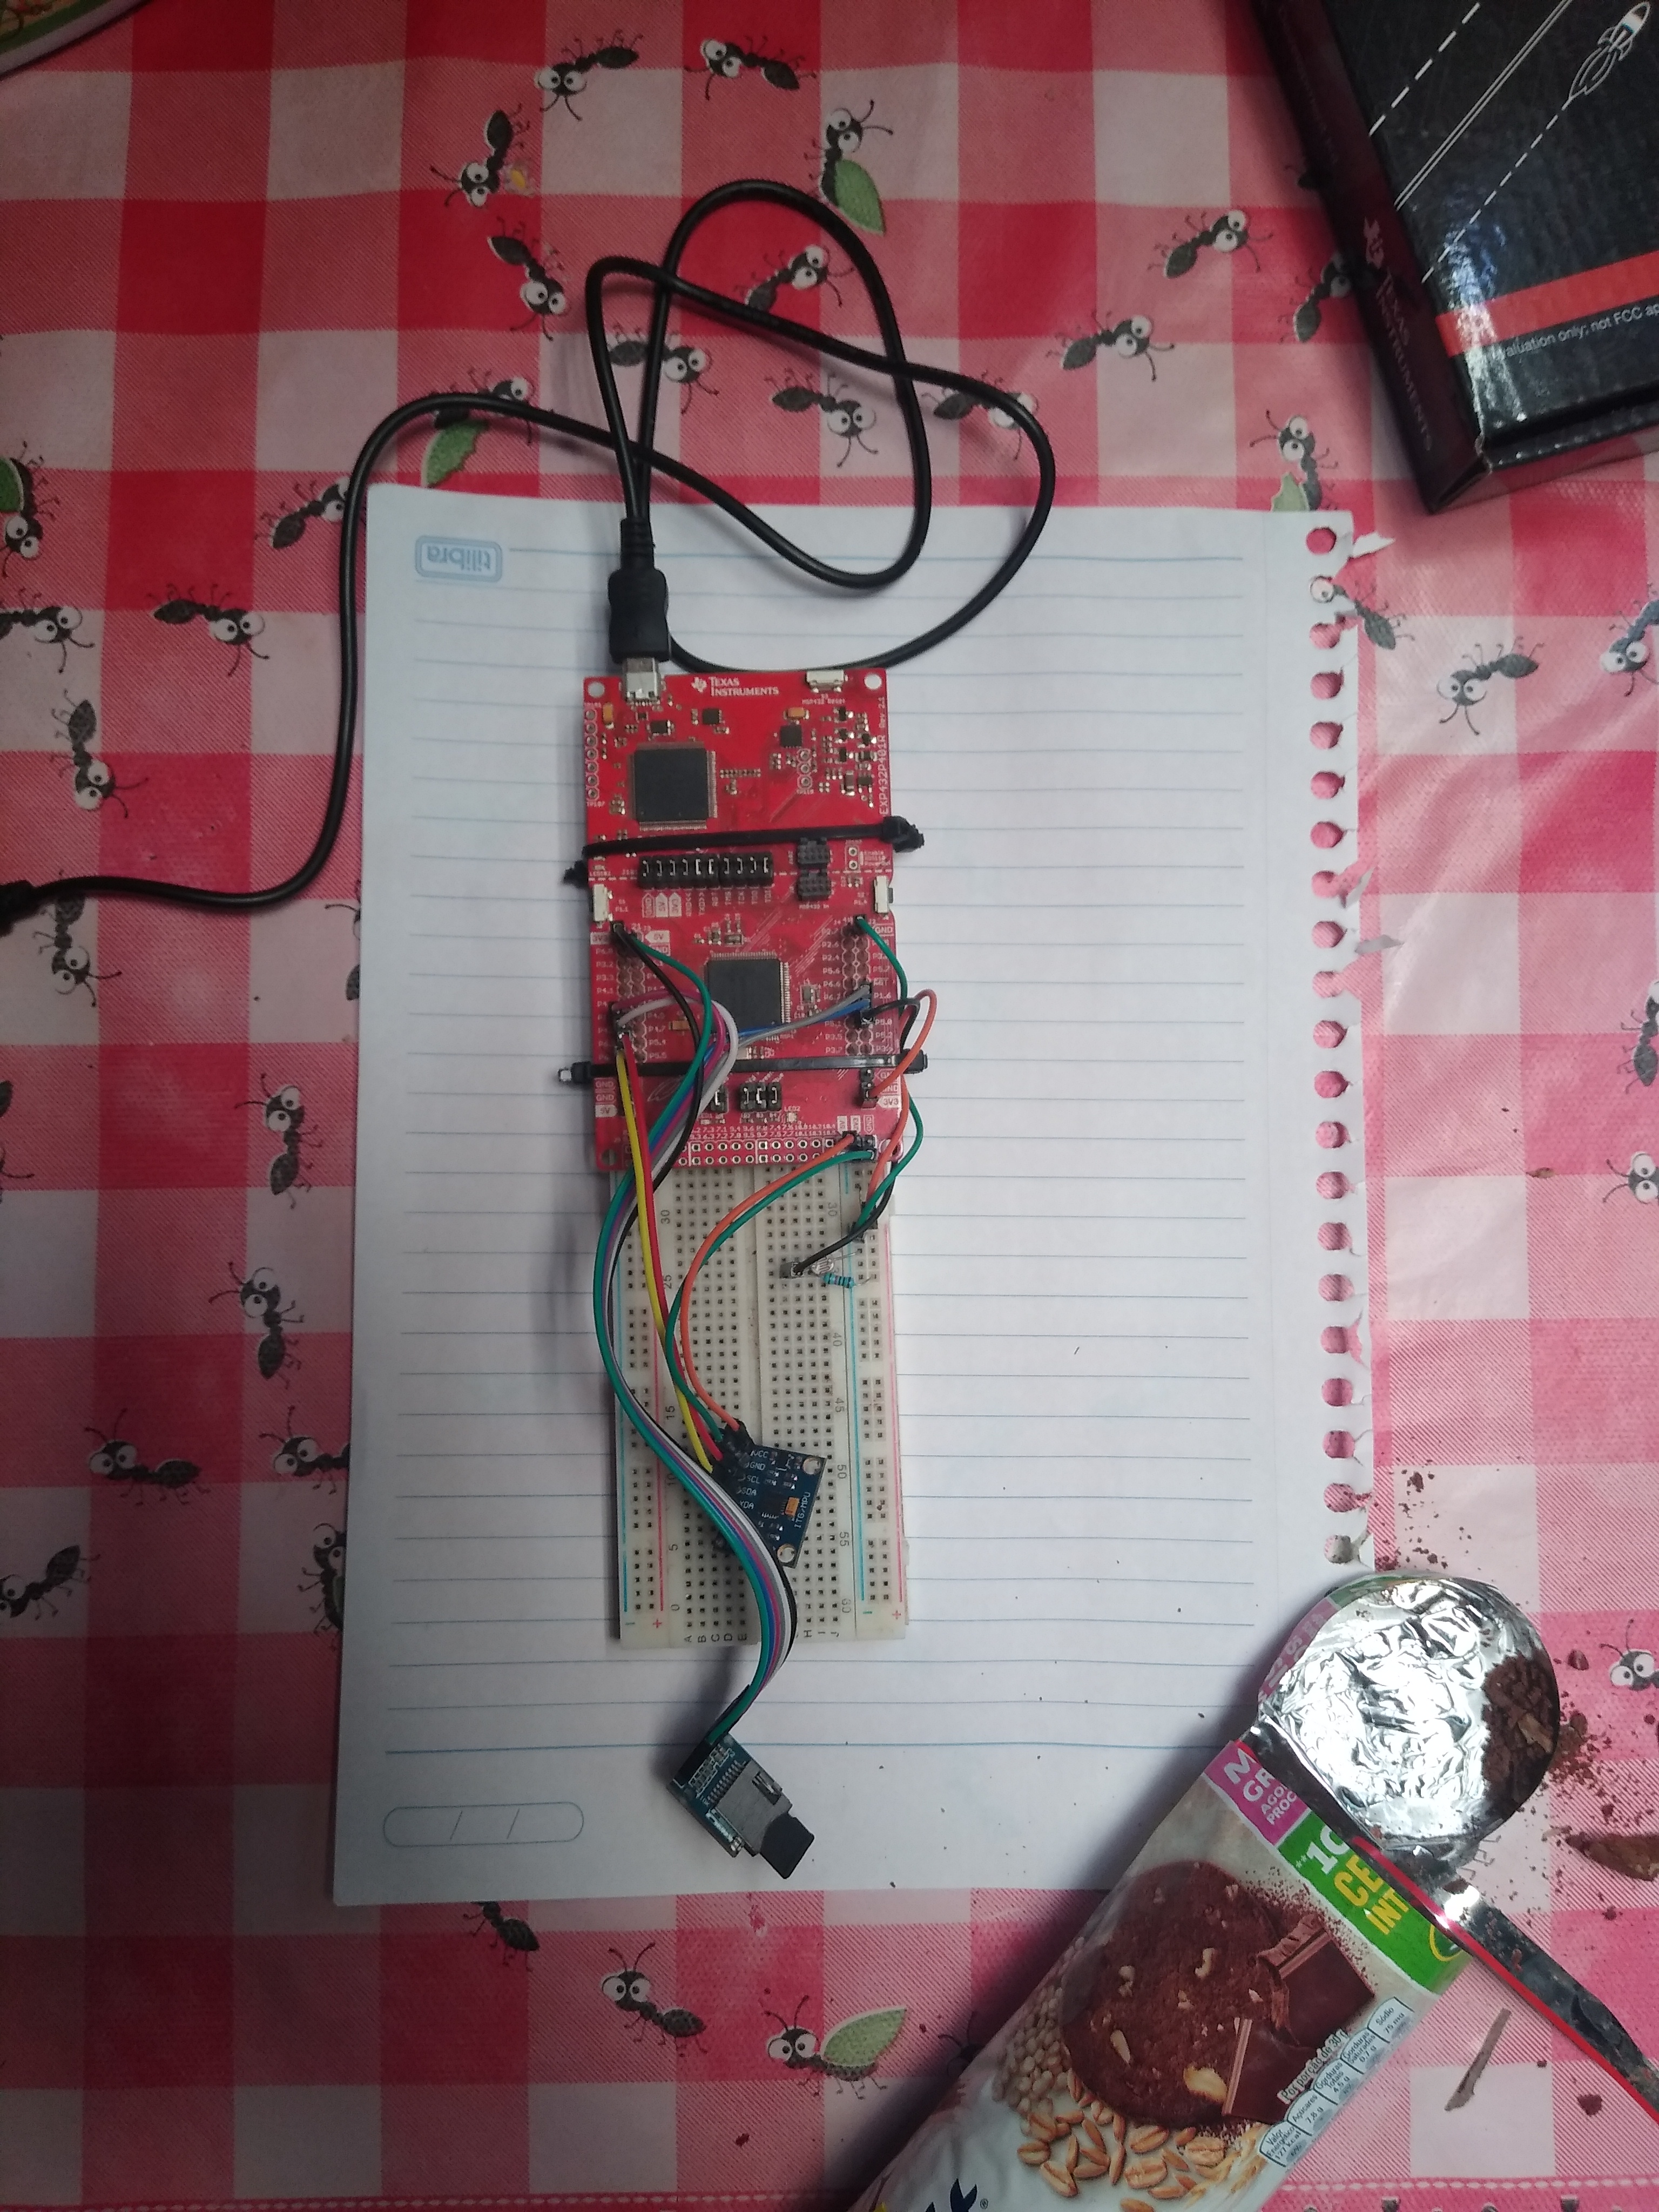
\includegraphics[keepaspectratio=true,scale=0.15]{figuras/protoboard.png}
	
	\label{proto}
\end{figure}

\section{Modos de Operação}

Para facilitar o entendimento da maquina de estados e utilizou-se o software Tracealyzer
OBC-SW-R7

\begin{figure}[h]
	\centering
	\caption{Tracealyzer SnapShoot.}
	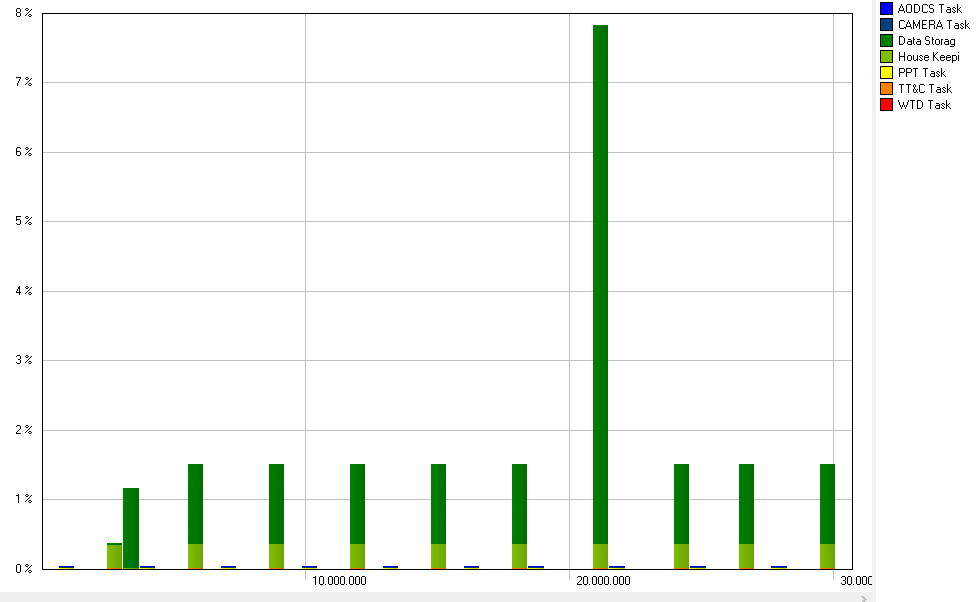
\includegraphics[keepaspectratio=true,scale=0.5]{figuras/trace_snapshoot.png}
	
	\label{operationMode}
\end{figure}

\section{Aquisição e Armazenamento de Dados}

O serviço de armazenamento de aquisição e armazenamento de dados é feito pelas Tasks HouseKeeping e DataStorage, respectivamente. 

Durante os testes realizados, os dados foram salvados em formato de strings, para facilitar o debug. Mas no futuro os dados serão armazenados conforme mostra o Apêndice \ref{apendiceb}, pois o armazenamento será muito mais eficiente e rápido. 

O pacote de telemetria especificado para o teste seguia a forma mostrada abaixo. Durante os testes houveram algumas falhas para armazenar os tempo relativo no computador de bordo. Alguns valores tiveram valor nulo.

\begin{figure}[h]
	\centering
	\caption{Formato do Pacote de Telemetria.}
	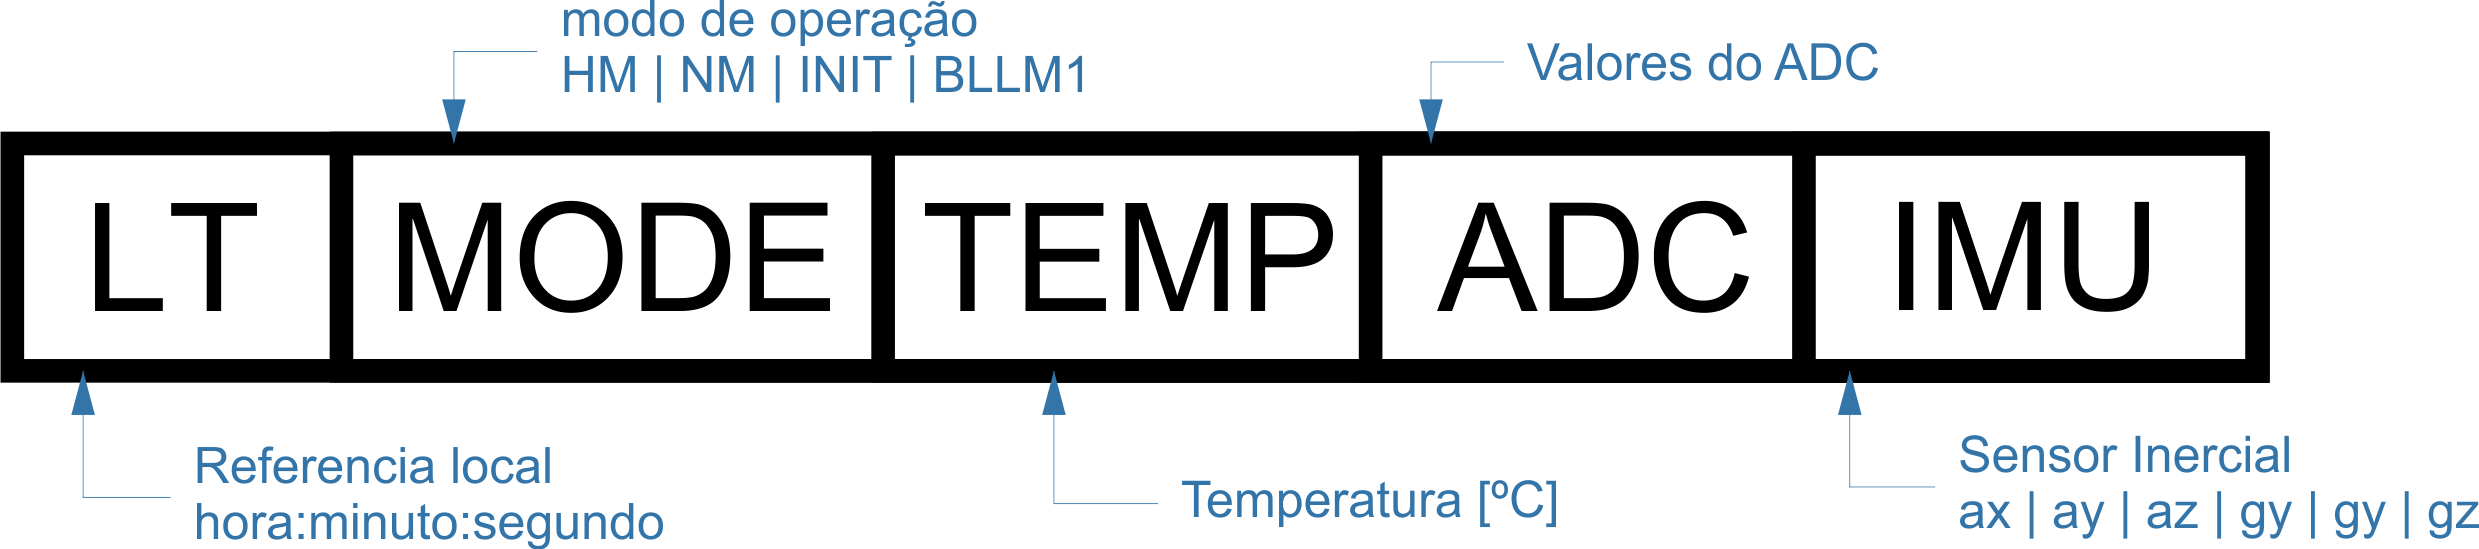
\includegraphics[keepaspectratio=true,scale=0.5]{figuras/telemetryPacket.png}
	
	\label{telemetryPacket}
\end{figure}

Todos os requisitos pertinentes à aquisição e armazenamento forma cumpridos, conforme mostra a Tabela \ref{table_Aquis}. Vale a pena ressaltar que o requisito \textit{OBC-H-R1} pede que os dados os dados dos subsistemas e Camera sejam armazenados. Ate o presente momento os subsitemas nao foram finalizados e o aluno enfrentou dificuldade para desenvolver o driver para a comunicação com a camera. 

\begin{longtable}[c]{clcl}
	\caption{Requisitos referentes à aquisição e armazenamento de dados.}
	\label{table_Aquis}\\
	\cline{1-2}
	\textbf{Número do Requisito} & \textbf{Descrição do Requisíto}                                                                                                                                                                                                                                                                   & \textbf{} & \multicolumn{1}{c}{\textbf{}} \\ \cline{1-2}
	\endfirsthead
	%
	\endhead
	%
	OBC-H-R1                     & \begin{tabular}[c]{@{}l@{}}OBC deve realizar a aquisição dos seguintes dados: Temperatura;\\ Tensão e Corrente consumidas pelo sistema; Sensor Inercial;Dados\\ dos demais subsistemas do CubeSat; Payload (Imagens da Câmera).\end{tabular}                                                      &           &                               \\
	OBC-H-R7                     & Possuir armazenamento não volátil de dados.                                                                                                                                                                                                                                                       &           &                               \\
	OBC-SW-R1                    & \begin{tabular}[c]{@{}l@{}}O OBC deve armazenar os seguintes dados a cada um segundo: Imagens \\da Carga Útil e informações temporais e espaciais das imagens;\\ Temperatura do sistema; Tensão e Corrente consumidas pelo sistema;\\ Atitude do CubeSat; Resposta de cada subsistema.\end{tabular} &           &                               \\
	OBC-SW-R3                    & O OBC deve realizar um log de eventos do sistema.                                                                                                                                                                                                                                                 &           &                               \\ \cline{1-2}
	&                                                                                                                                                                                                                                                                                                   &           &                               \\
	&                                                                                                                                                                                                                                                                                                   &           &                               \\
	&                                                                                                                                                                                                                                                                                                   &           &                               \\
	&                                                                                                                                                                                                                                                                                                   &           &                              
\end{longtable}

A Figura \ref{telemetryData} mostra os dados armazenados durante os testes.

\begin{figure}[h]
	\centering
	\caption{Dados da telemetria armazenados no cartão de memoria.}
	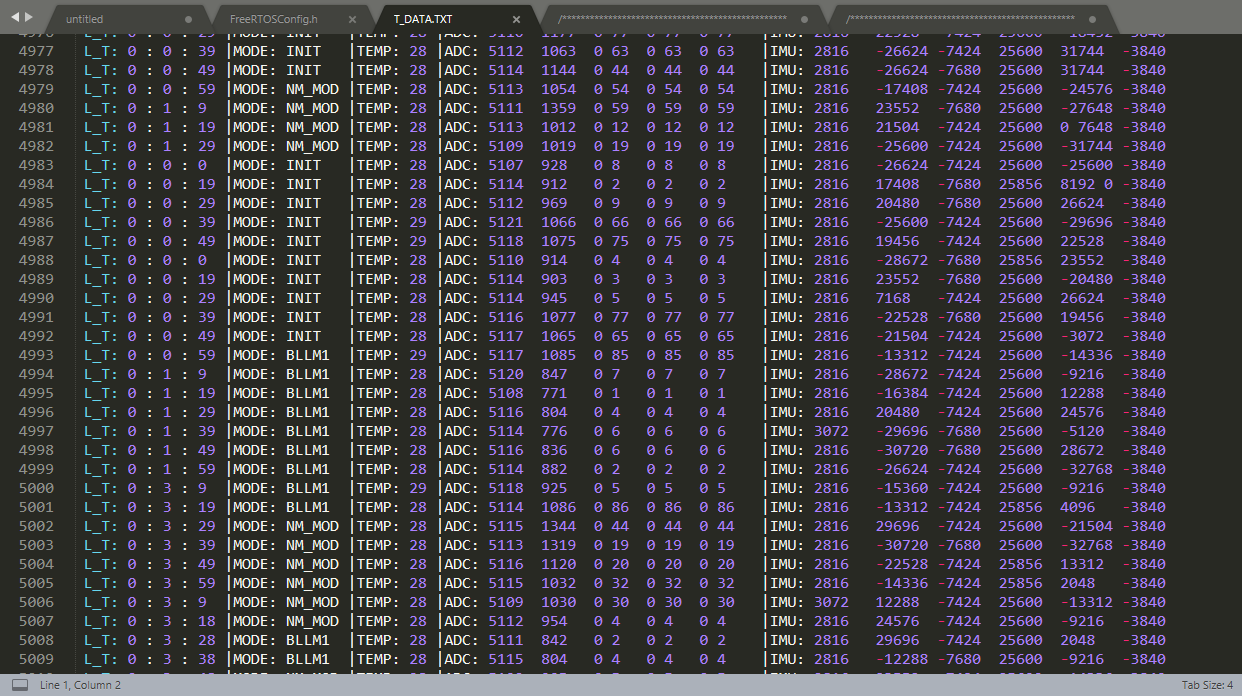
\includegraphics[keepaspectratio=true,scale=0.50]{figuras/telemetryData.PNG}
	
	\label{telemetryData}
\end{figure}

\section{Sistema Anti Travamento}
OBC-H-R2
OBC-H-R6
OBC-SW-R8

O sistema possui watchdog pelo FreeFrtos, por hardware via MSP432 e externo pelo STD.

\section{Consumo}

Um dos critérios mais importantes para o design de um OBC é o consumo energético em varias condições de operação. Ainda é mais importante nanosatelites onde a fonte de energia é limitada pela área dos painéis solares. 

Os testes de consumo foram realizados utilizando a ferramenta \textit{EnergyTracer} do \textit{Code Composer Studio}. Essa ferramenta mede a corrente sendo consumida no barramento JTAG/SW, sendo assim ela permite calcular a corrente de todos os módulos/sensores alimentados pela launchpad. 

Para simular o \textit{EPS} do CubeSat, foi utilizado um \textit{photoresistor} para indicar o nível de bateria. Houveram tres baterias de teste de cinco minutos, um para cada estado. Os dados do consumo de cada um esta presente na tabela 1.

Comparando o estado de nominal com o estado de hibernação, observa-se que houve uma economia de mais de 40\textperthousand aumentando a vida da bateria em dois dias. A Figura mostra a comparação em forma gráfica, hibernação em azul e nominal em amarelo.

\begin{figure}[h]
	\centering
	\caption{Comparação entre os Modos de hibernação (azul) e Nominal (amarelo).}
	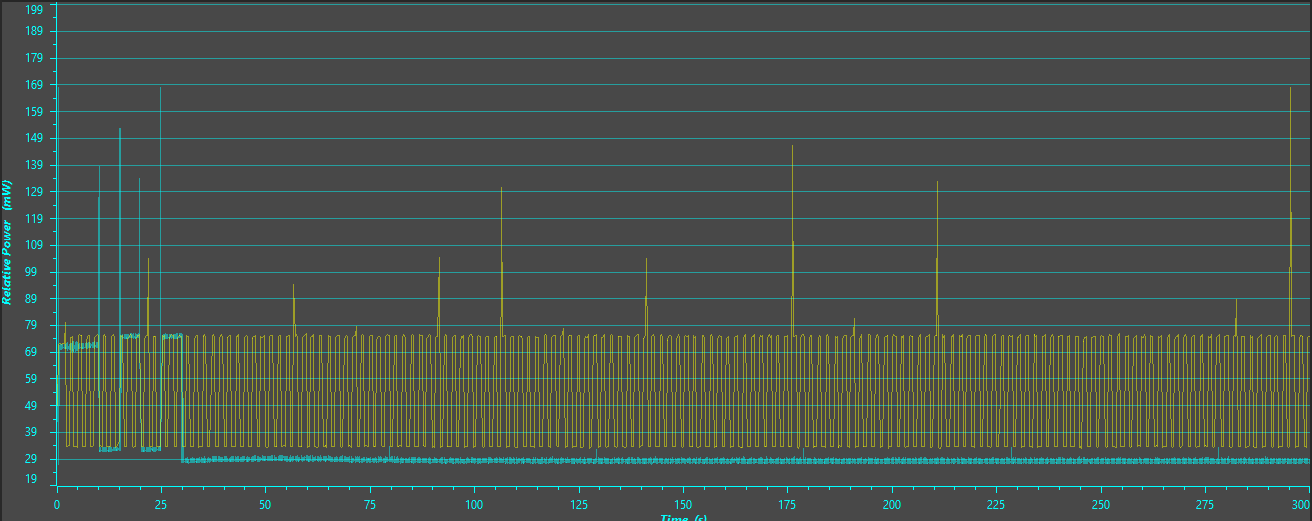
\includegraphics[keepaspectratio=true,scale=0.470]{figuras/hibernatexNormal.PNG}
	
	\label{hibernatexNormal}
\end{figure}

Não foi possível concluir a mesma melhoria comparando o modo de baixo consumo com o modo de hibernação. Houve apenas uma economia de 9\textperthousand,0.6 dias. Esse fato ocorre por que o modo de hibernação não está completamente otimizado. A fonte de sincronismo durante esse estado ainda continua sendo 48MHz. O ideal seria utilizar o clock externo de 32KHz para realizar as interrupções do kernel. Infelizmente devido à inexperiência do aluno com o FreeRTOS, não foi possível adicionar uma segunda fonte de sincronismo no modo de baixo consumo. A Figura mostra a comparação em forma gráfica, hibernação em azul e nominal em amarelo.

\begin{figure}[h]
	\centering
	\caption{Comparação entre os Modos de hibernação (azul) e Pouca Bateria (amarelo).}
	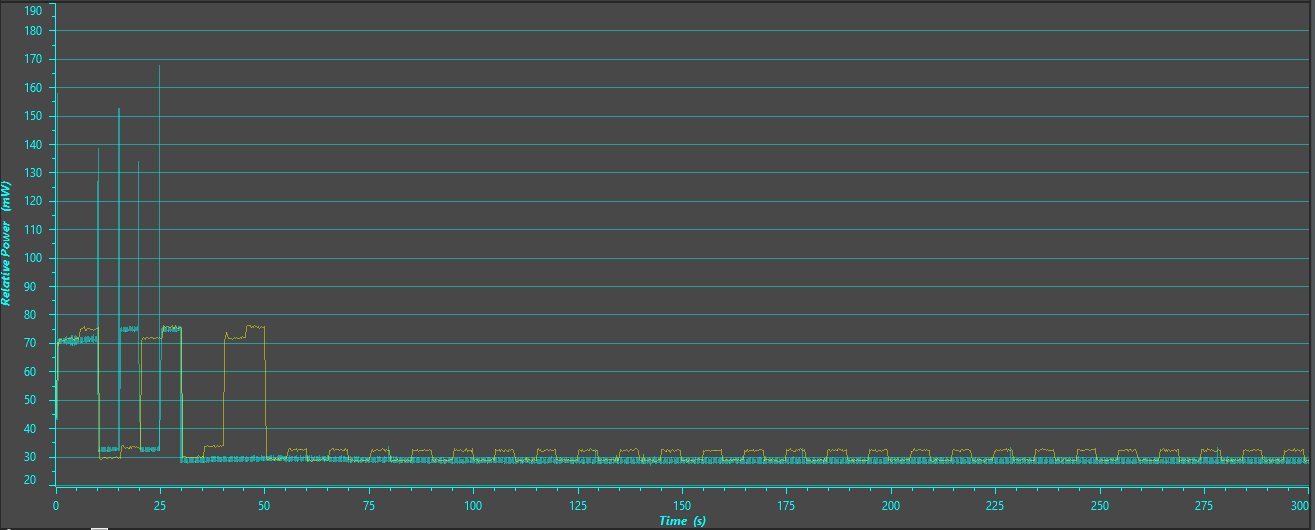
\includegraphics[keepaspectratio=true,scale=0.470]{figuras/hibernatexLBM.PNG}
	
	\label{hibernatexLBM}
\end{figure}

Apesar de não ter sido implementado o clock de baixa frequência para o modo de hibernação, é possível confinar que o software embarcado consegue alterar o modo de operação dependendo de uma fonte externa. Sendo assim, o requisito OBC-SW-R7 foi cumprido.

Fazendo uma estimativa com os outros sensores/periféricos. A tabela abaixo mostra o consumo de cada componente, de acordo com cada fabricante

\hl{TABELA COMPARATIVA}


\chapter[CONCLUSÃO E RECOMENDAÇÕES]{CONCLUSÃO E RECOMENDAÇÕES}

\section{Conclusões}
Os objetivos da pesquisa foram alcançados em parte.
- houve o controle da câmera CMOS.
- Até o presente momento, a parceria está em fase de discussão. Sendo assim não foi possível realizar os teste com o PPT, mas o barramento ISA PC104 está com os pinos especificados para o realizar a interface.
- O sistema possui um nível considerável de segurança pois foram implementados o Watchdog via FreeRTOS, WTD via MSP432 e um WTD via Hardware. Possui um sensor contra alta corrente. Isso minimizará os riscos de se usar componentes COTS sem tolerância a radiação.
- X% dos requisitos foram alcançados. 
- O uso de requisitos de outras missões serviram como base para a realização do projeto, entretanto nos próximos trabalhos seria interessante realizar o estudo aprofundado dos requisitos da missão para que o projeto tenha mais. 
- Codesign. 
- MSP432 como solução de baixo consumo e processamento intermediário. 
- Uso do FreeRTOS como uma alternativa para um sistema operacional de baixo consumo e baixo processamento. 
- Foi possível constatar que a máquina de estados da missão foi realizada. O auxílio de ferramentas como o tracealyzer permitiu a otimização das tasks. Devido a escassez de tempo, não foi possível realizar o modo SAAFE MODE.
- Uso de ferramentas opensource.
- GitHub como plataforma de versionamento e disseminação da pesquisa. Isso ajuda a criar softwares que possam ser reutilizados em futuros projetos. Sem contar que o código fica versionado.
-Open source.
Os objetivos da pesquisa foram alcançados em parte.
- houve o controle da câmera CMOS.
- Até o presente momento, a parceria está em fase de discussão. Sendo assim não foi possível realizar os teste com o PPT, mas o barramento ISA PC104 está com os pinos especificados para o realizar a interface.
- O sistema possui um nível considerável de segurança pois foram implementados o Watchdog via FreeRTOS, WTD via MSP432 e um WTD via Hardware. Possui um sensor contra alta corrente. Isso minimizará os riscos de se usar componentes COTS sem tolerância a radiação.
- Xporcento dos requisitos foram alcançados. 
- O uso de requisitos de outras missões serviram como base para a realização do projeto, entretanto nos próximos trabalhos seria interessante realizar o estudo aprofundado dos requisitos da missão para que o projeto tenha mais. 
- Codesign. 
- MSP432 como solução de baixo consumo e processamento intermediário. 
- Uso do FreeRTOS como uma alternativa para um sistema operacional de baixo consumo e baixo processamento. 
- Foi possível constatar que a máquina de estados da missão foi realizada. O auxílio de ferramentas como o tracealyzer permitiu a otimização das tasks. Devido a escassez de tempo, não foi possível realizar o modo SAAFE MODE.
- Uso de ferramentas opensource.
- GitHub como plataforma de versionamento e disseminação da pesquisa. Isso ajuda a criar softwares que possam ser reutilizados em futuros projetos. Sem contar que o código fica versionado.
-Open source.

\section{Recomendações}

- Soldagem dos componentes. E teste da placa.
- Projeto subestimado. Precisa de mais pessoas. Utilizar o projeto para a realização de um laboratório de aplicações espaciais. 
- Parcerias com outras universidades/LAICAnSat/Inpe;
- Realizar o teste com balão estratosférico.
- Coleta de requisitos.
- Sistema para mitigar falhas.
- A possibilidade de usar componentes SMD menores.
- Otimização do port.h e a utilização de uma fonte de clock de 32KHz para SysTick, com o intuito de usar no modo de hibernação. 



